\documentclass{beamer} % [aspectratio=169]
 
\usepackage[utf8]{inputenc}
\usepackage[danish]{babel}
\usepackage{natbib}
\usepackage{graphicx}
\usepackage{amsmath}
\usepackage{amsfonts}
\usepackage{amssymb}
\usepackage{amsthm}
\usepackage{tikz}
\usepackage{verbatim}
\newcommand{\R}{\mathbb{R}}
\newcommand{\CC}{\mathbb{C}}
\newcommand{\F}{\mathbb{F}}
\newcommand{\K}{\mathbb{K}}

\newcommand{\borel}{\mathcal{B}}
\newcommand{\sE}{\mathcal{E}}

\newcommand{\isomorph}{\cong}

\newcommand{\fat}[1]{\mathbf{#1}}
\newcommand{\curly}[1]{\{#1\}}
\newcommand{\para}[1]{\left(#1\right)}
\newcommand{\makeset}[2]{\curly{#1 \mid #2}}
\newcommand{\makesetcolon}[2]{\curly{#1 \, : \, #2}}
\newcommand{\openint}[2]{\mathopen]#1, #2\mathclose[}
\newcommand{\closedint}[2]{\mathopen[#1, #2\mathclose]}
\newcommand{\fracp}[2]{\left(\frac{#1}{#2}\right)}
\newcommand{\abs}[1]{\left\lvert #1 \right\rvert}
\newcommand{\norm}[1]{\left\lVert #1 \right\rVert}
\newcommand{\ip}[2]{\langle #1, #2\rangle}
\newcommand{\generator}[1]{\langle#1\rangle}
\newcommand{\paraip}[2]{\left\langle #1, #2\right\rangle}
%\newcommand{\comment}[1]{\quad \para{\text{#1}}}

\newcommand{\longpause}{\break \break \pause}

% CompGeo
\DeclareMathOperator{\dist}{dist}
\DeclareMathOperator{\Vor}{Vor}
\DeclareMathOperator{\VorG}{Vor_{G}}
\DeclareMathOperator{\bi}{bi}

% superior (?) pause command
\makeatletter
\newcommand{\Pause}[1][]{\unless\ifmeasuring@\relax
\pause[#1]%
\fi}
\makeatother

\usetheme{Madrid}

\title{Specialeforsvar}
\author{Johannes Jensen}
\institute{Aarhus Universitet}
\date{\today}
 
\begin{document}
 
\frame{\titlepage}

\begin{comment}

\begin{frame}
\pause
\[
	\huge\text{Introduktion}
\]
\end{frame}

\begin{frame}
\pause
\[
	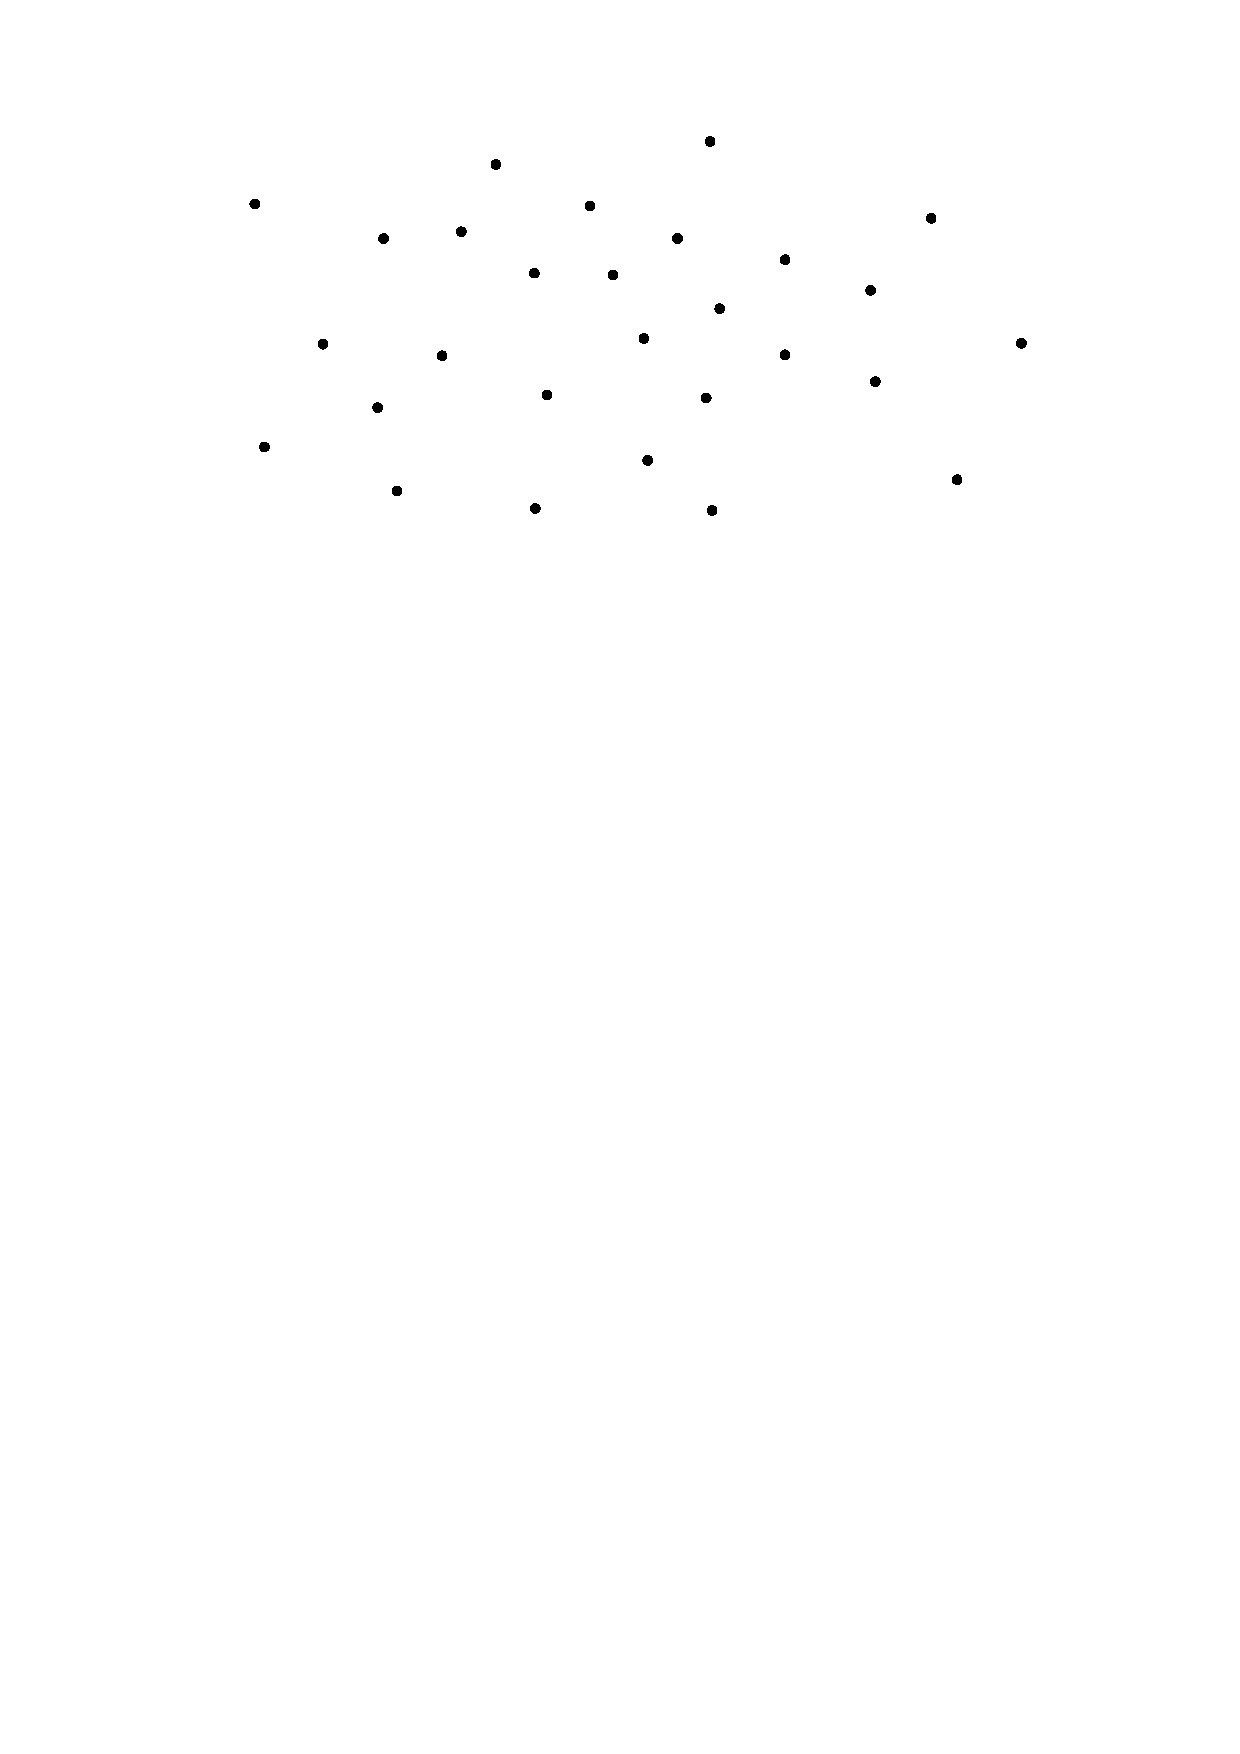
\includegraphics[scale=0.7]{images/intro_without_diagram}
\]
Lad $P = \curly{p_1, p_2, \ldots, p_n} \subset \R^2$ betegne en endelig mængde af \textit{sites}.
\end{frame}

\begin{frame}
\[
	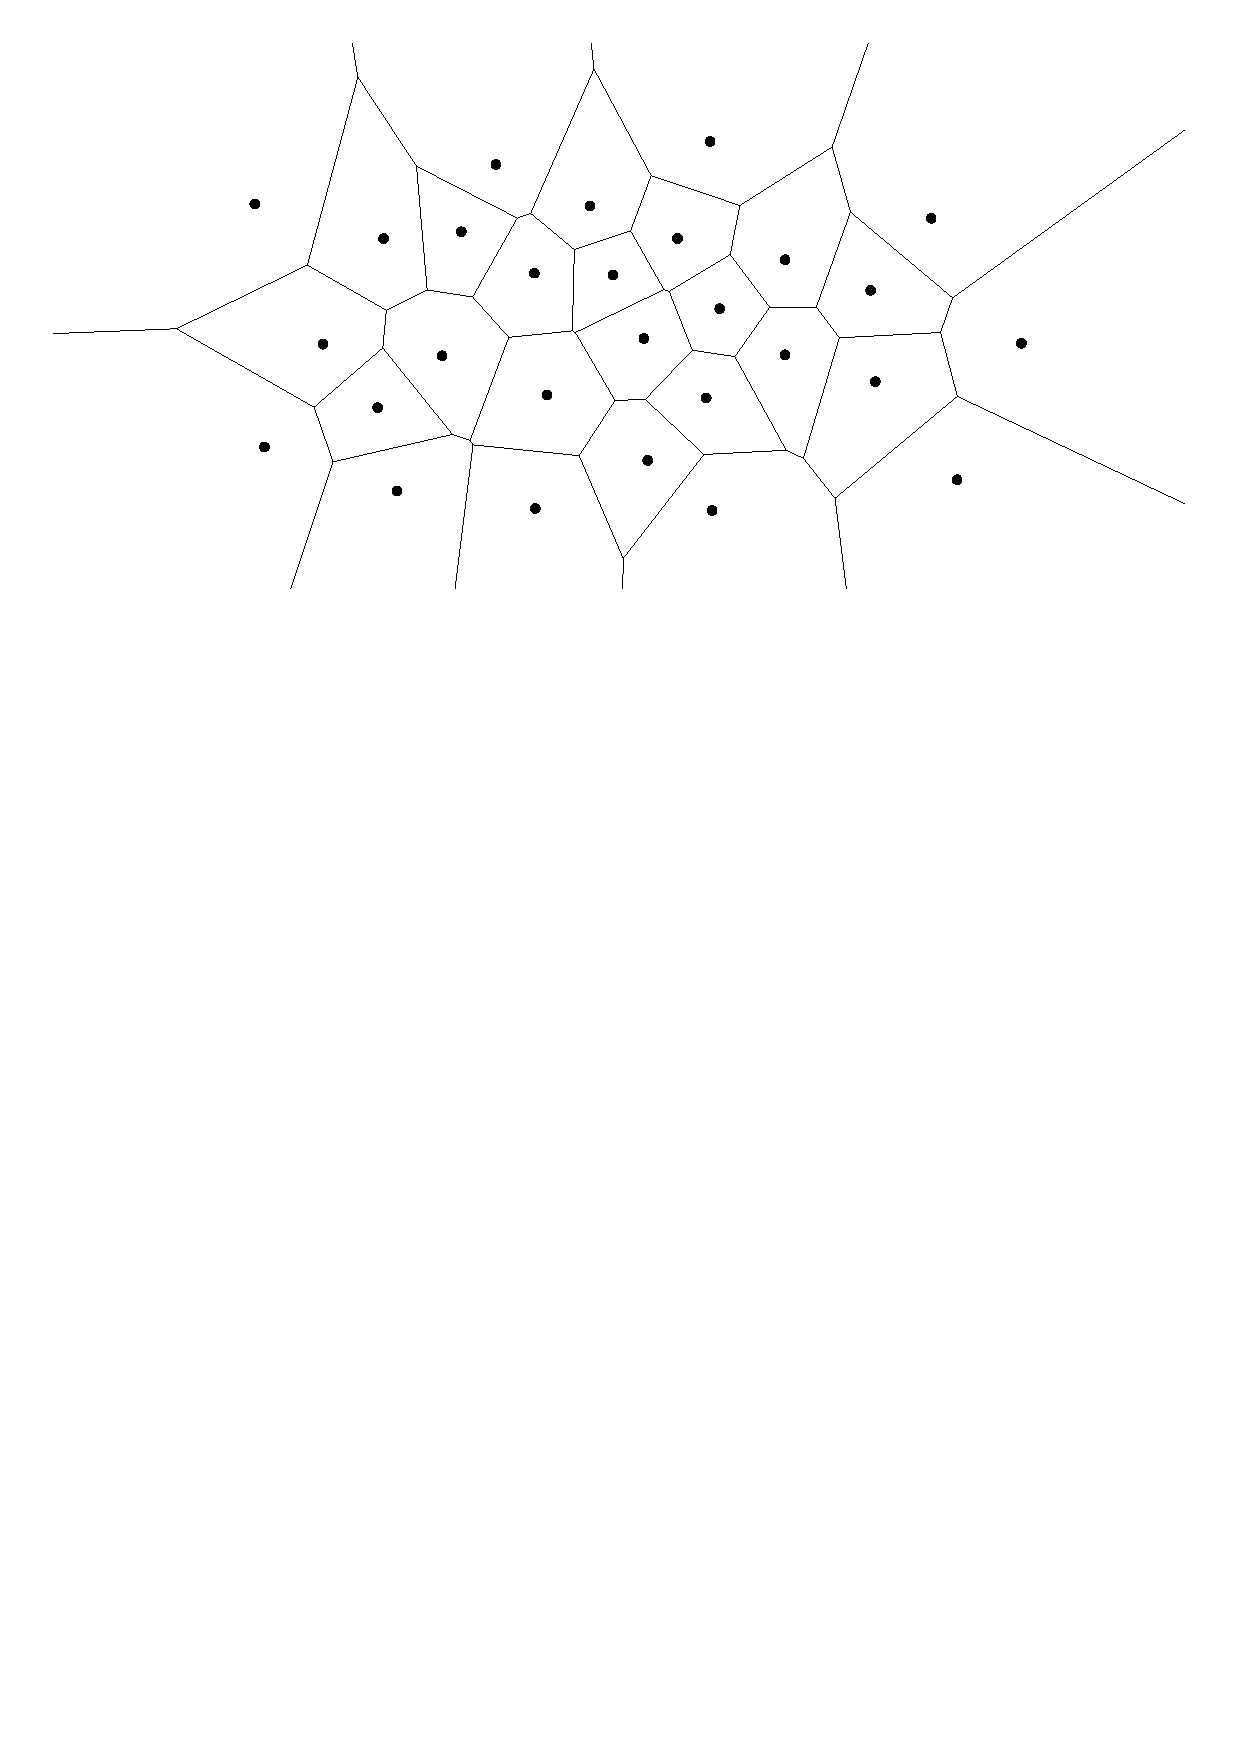
\includegraphics[scale=0.7]{images/intro_with_diagram}
\]
Vi ønsker så at beregne $\Vor(P)$, \textit{Voronoi diagrammet} for $P$.
\end{frame}

\begin{frame}
\[
	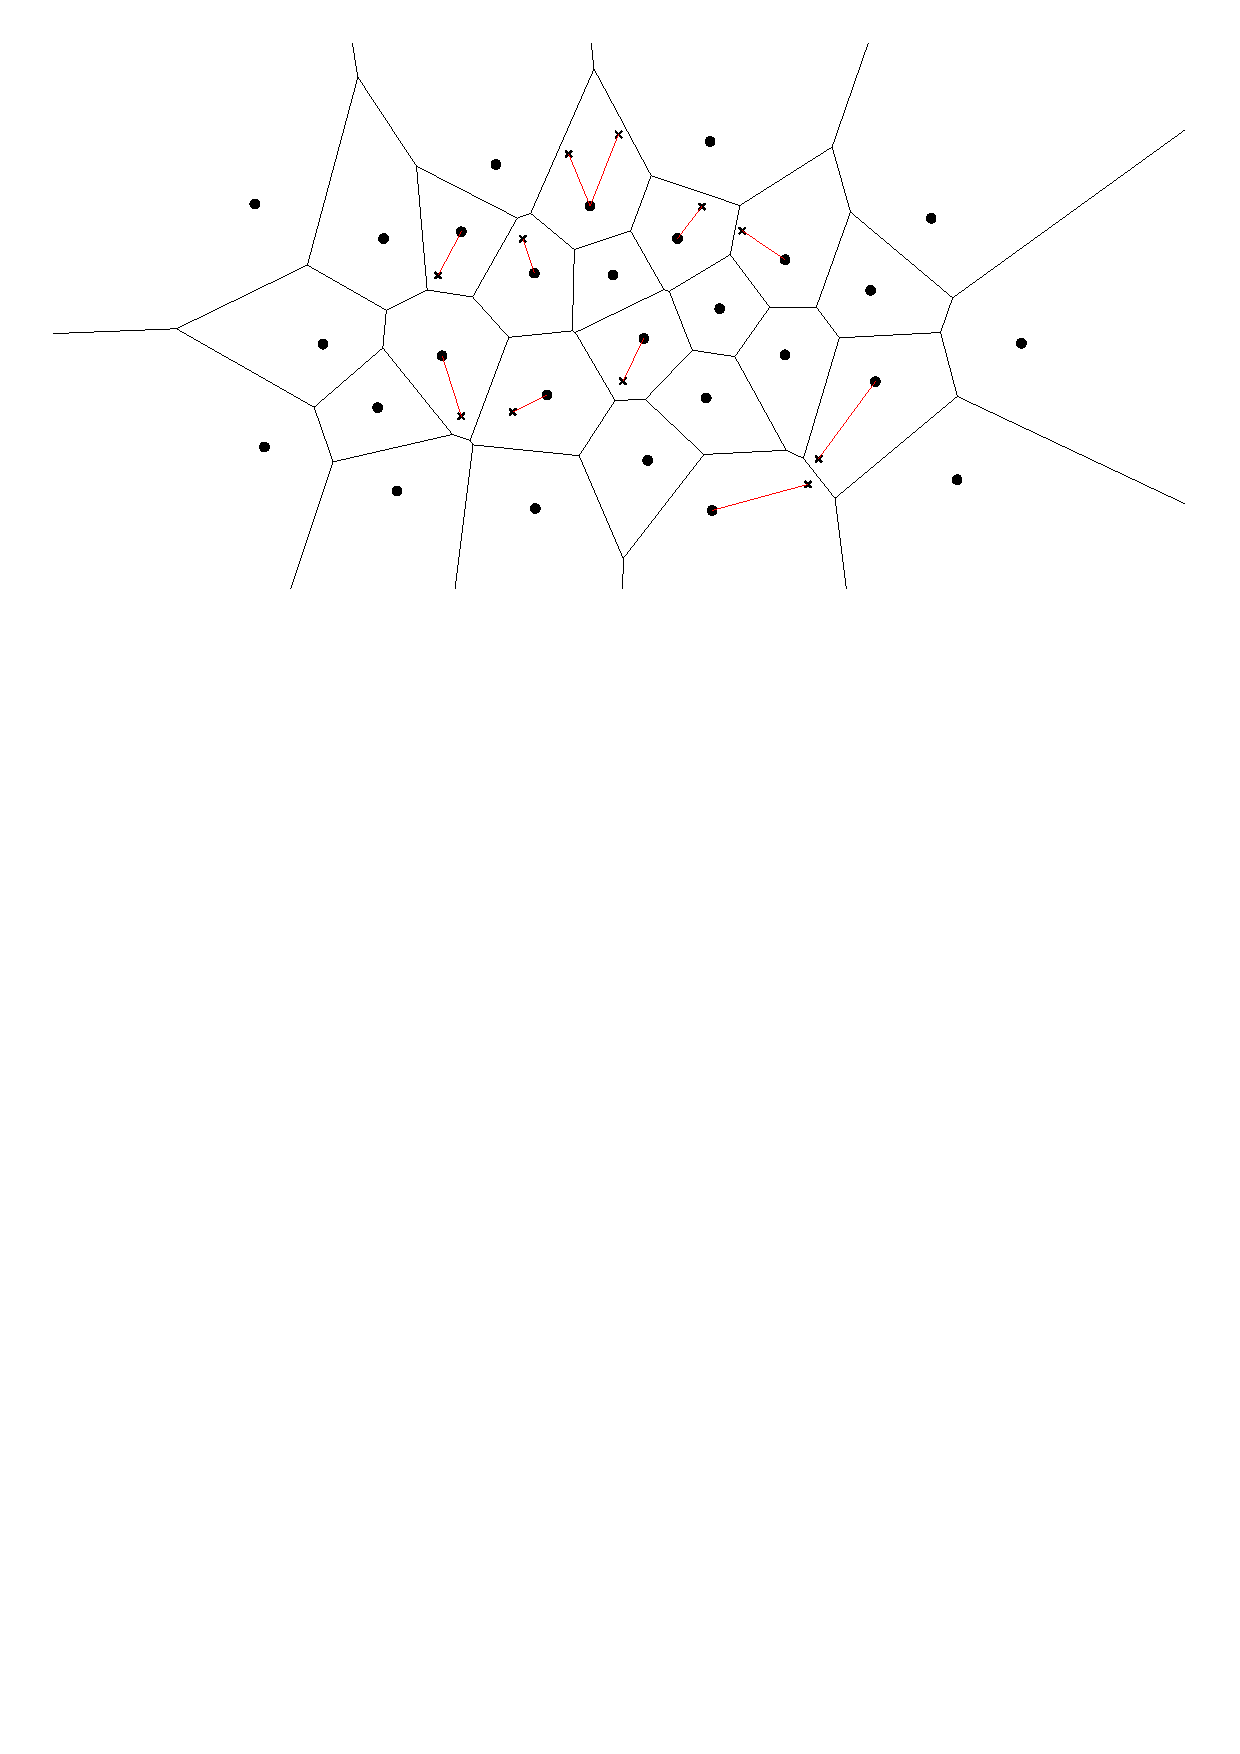
\includegraphics[scale=0.7]{images/intro_distances}
\]
Hvad kan Voronoi diagrammet? Givet et $\times$ i en \textit{Voronoi celle} angiver diagrammet hvilket punkt fra $P$ som er tættest på!
\end{frame}

\begin{frame}
\pause
Men hvordan beregner man det?
\longpause
Man bruger en \textit{sweep line algorithm}! (En fejende linje algoritme...?)
\longpause
Demo tid!
\end{frame}

\begin{frame}
\pause
Hvorfor virker det?
\longpause
\[
	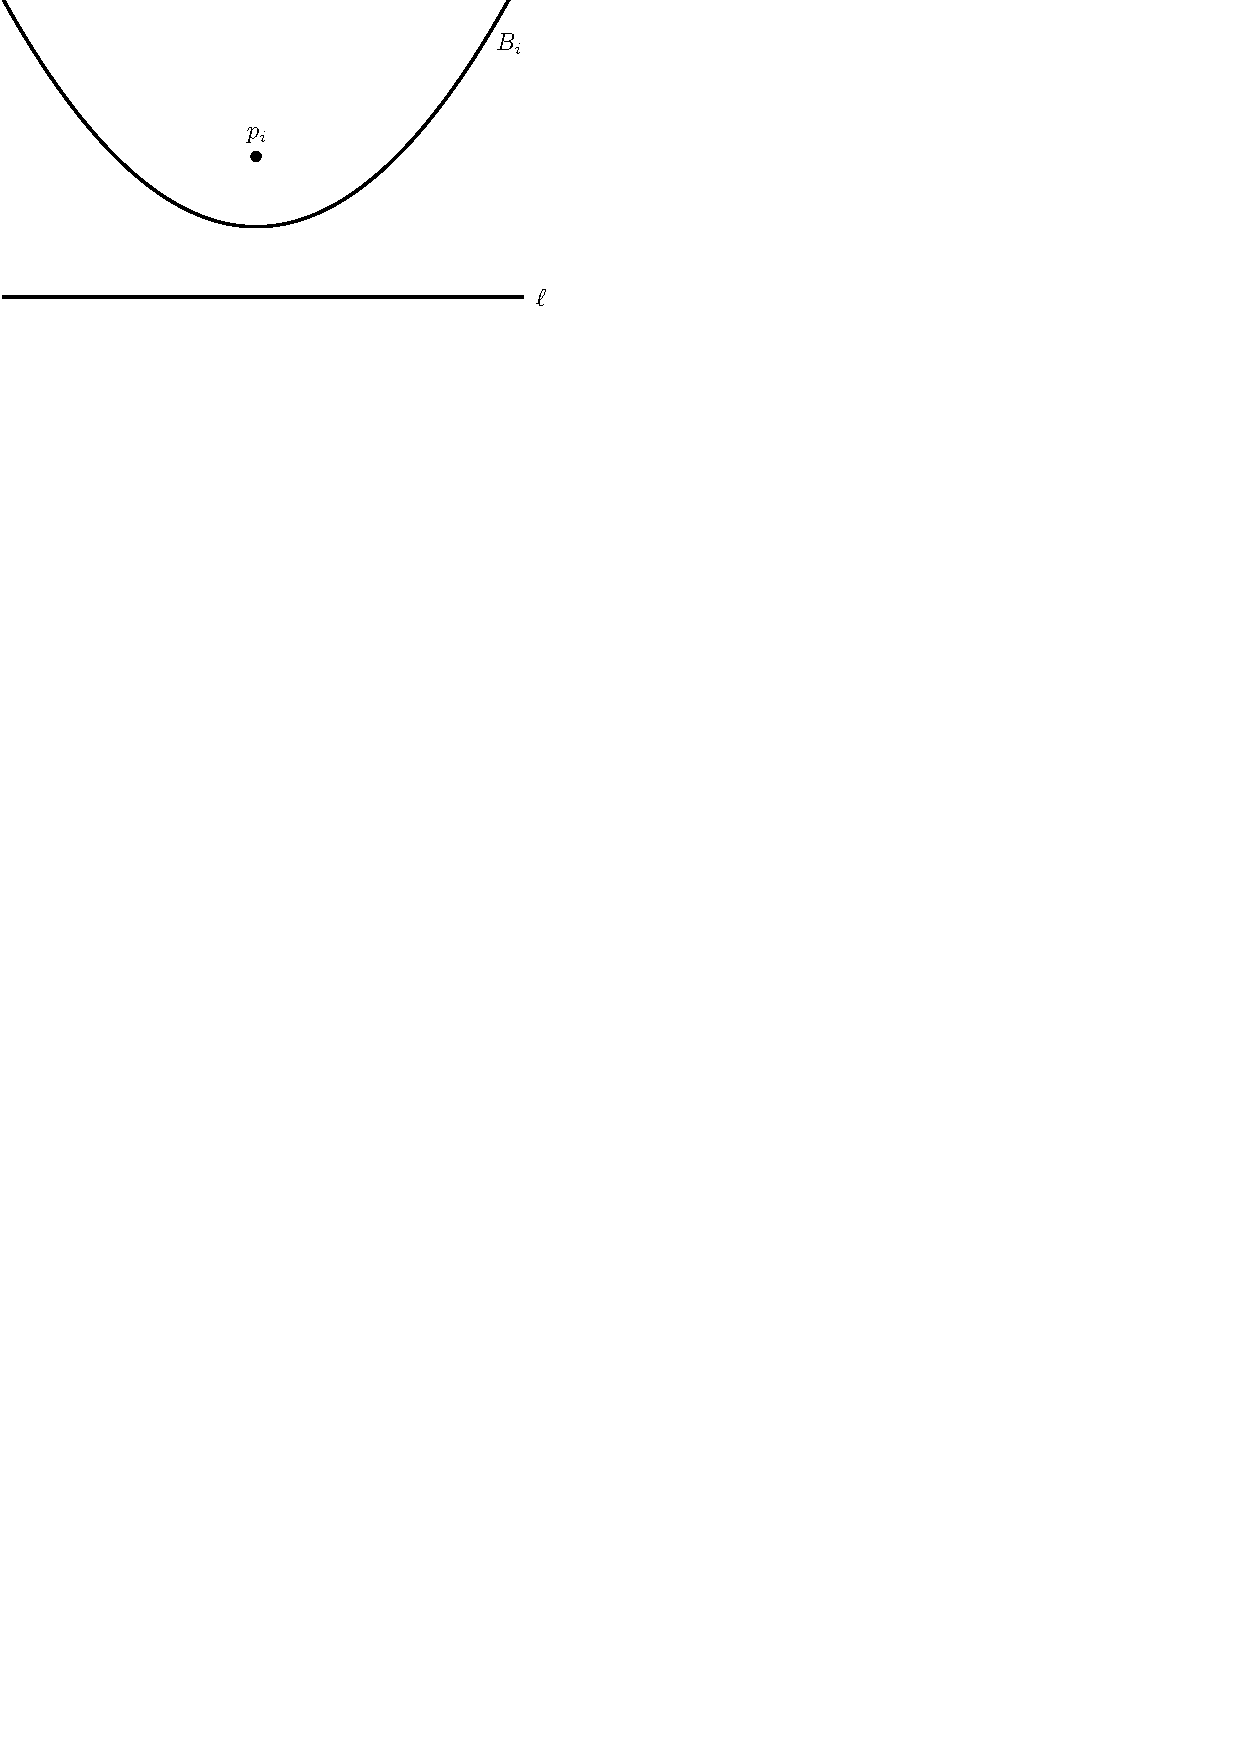
\includegraphics[scale=0.9]{../images/hyperbola_intro}
\]
Vi kan separere ethvert site $p_i \in P$ og vores sweep line $\ell$ med en andengradskurve $B_i$\pause, således at for alle $q \in B_i$ så $\dist(q, p_i) = \dist(q, \ell)$.
\end{frame}

\begin{frame}
\pause
Vi kan så gøre dette for alle sites i $P$, men vi beholder kun de dele af kurverne som ligger tættest på $\ell$:
\[
	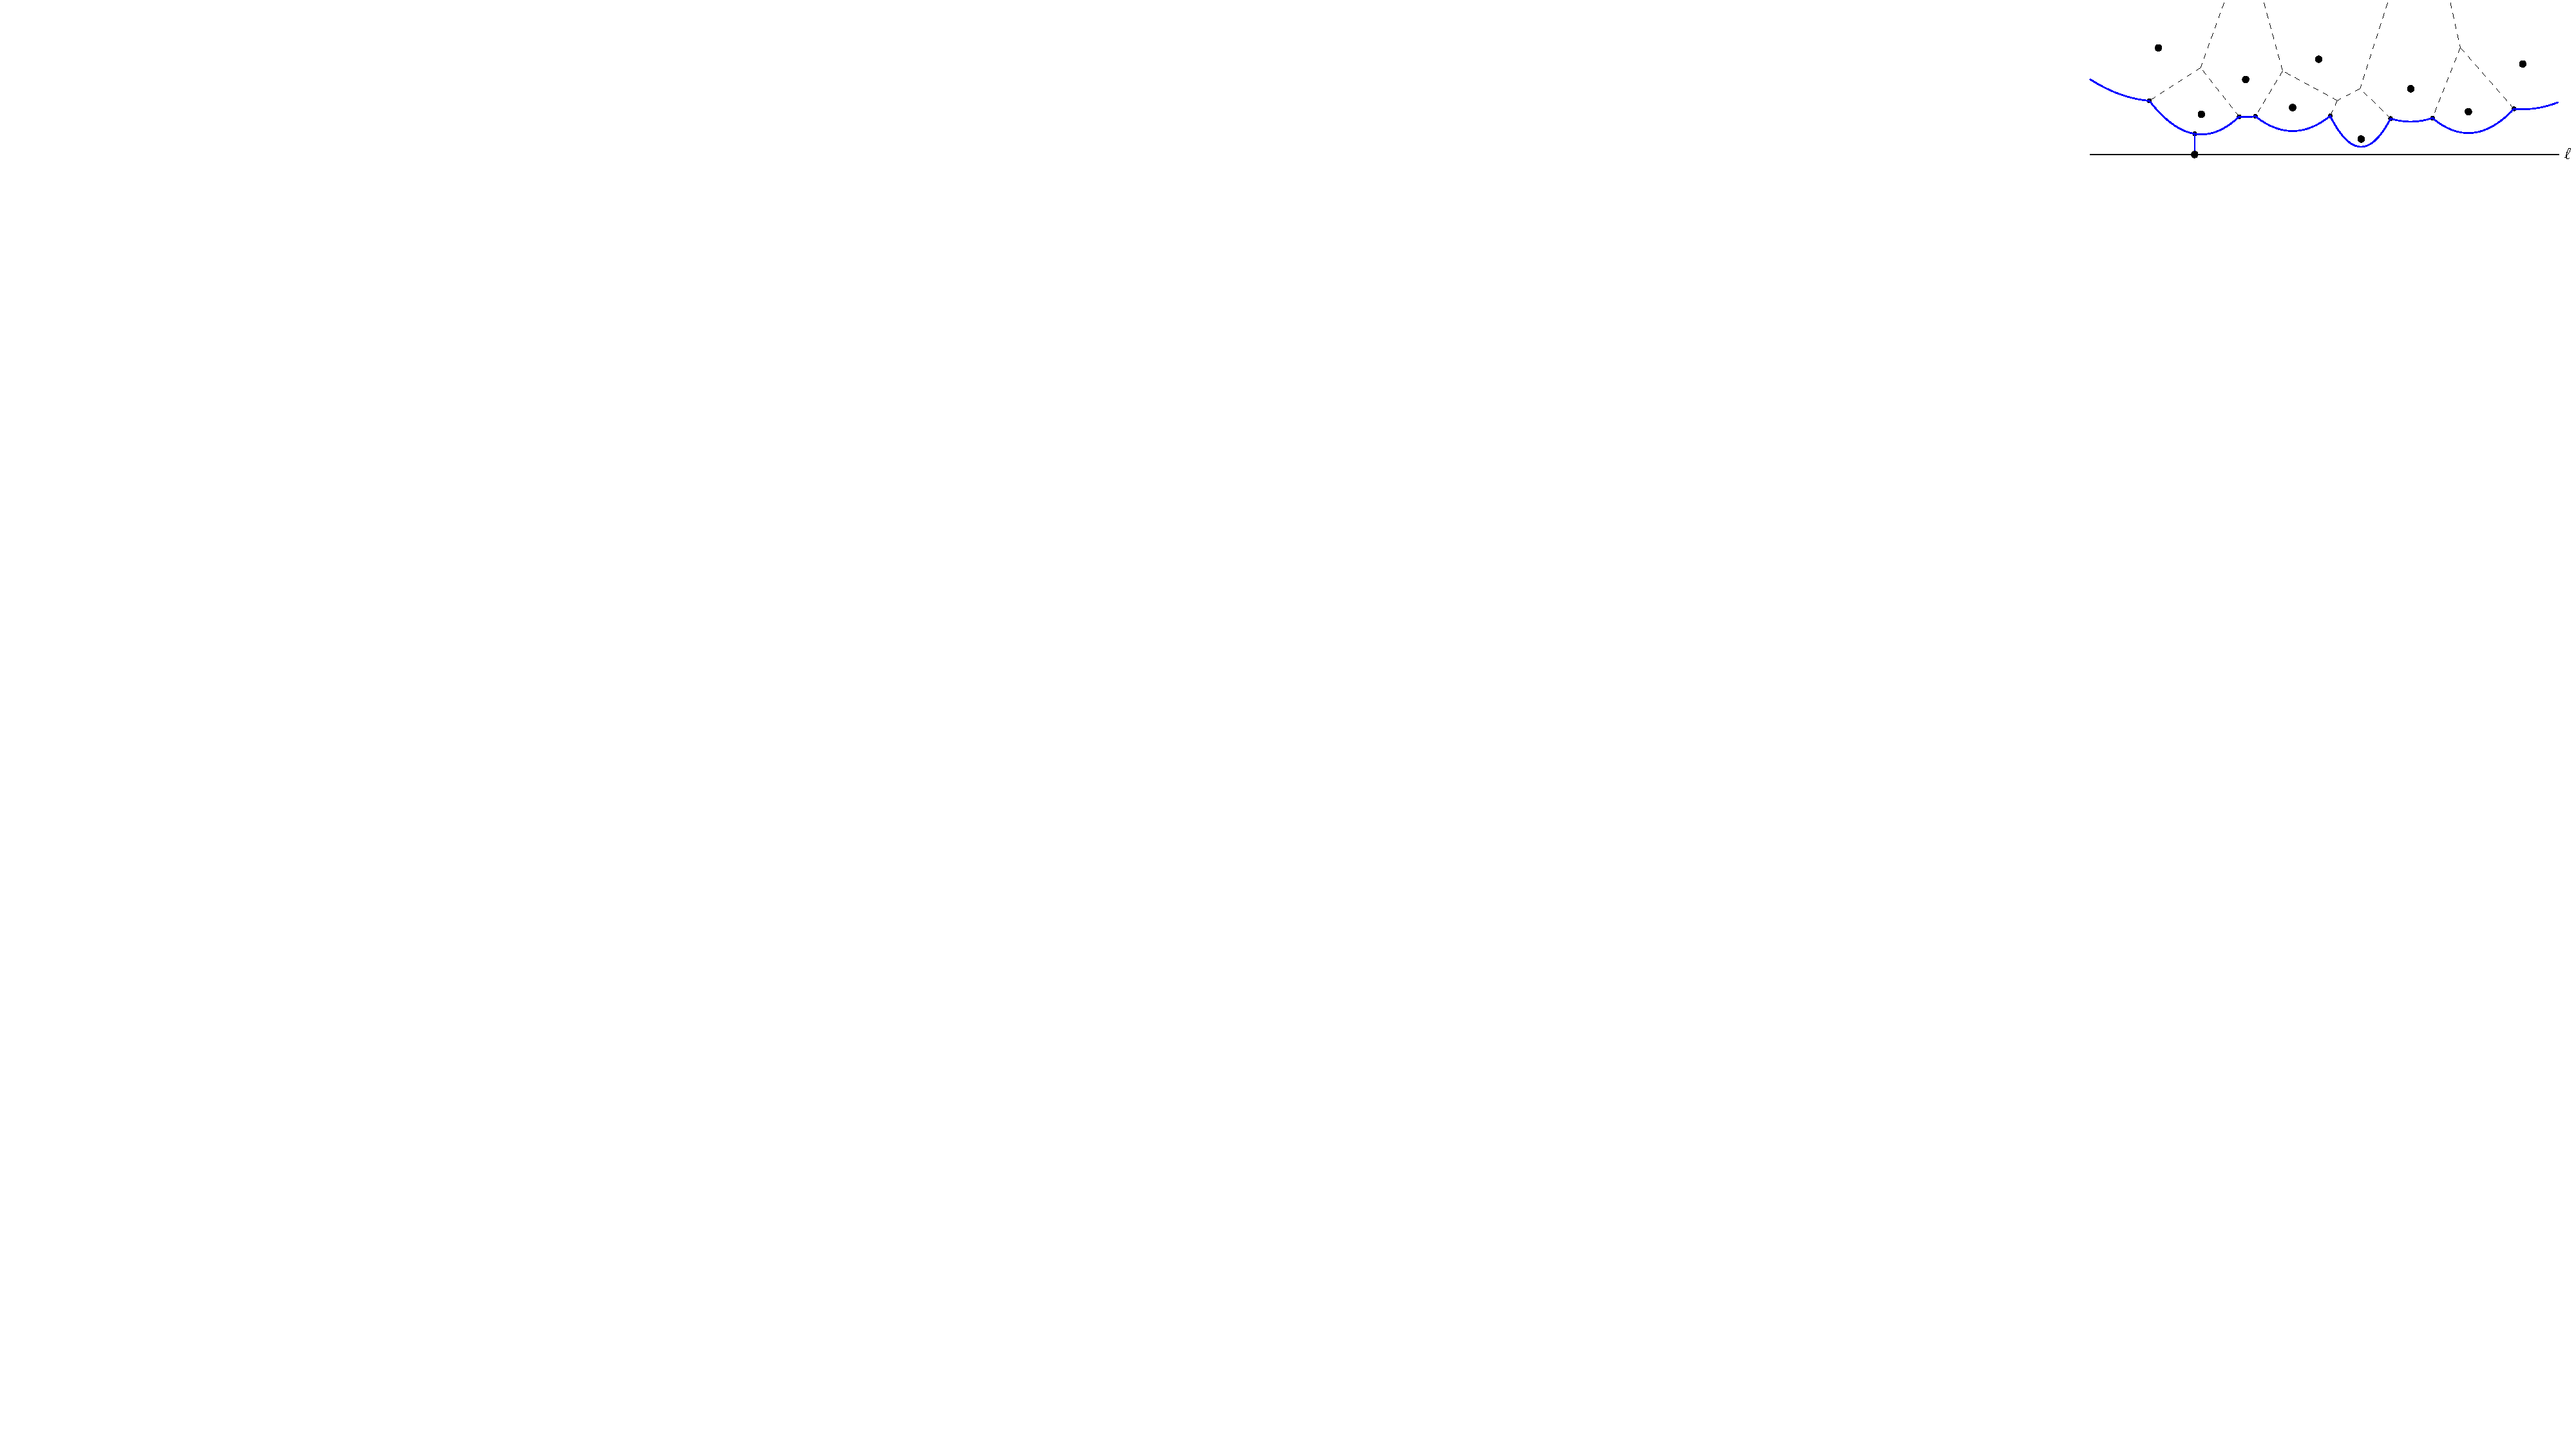
\includegraphics[scale=0.8]{../images/beachline}
\]
\pause
Den blå kurve kalder vi for \textit{the beach line} (kystlinjen) for $\ell$ mht. $P$.
\longpause
At sweep line metoden virker følger så fra at skæringerne mellem forskellige $B_i$ og $B_j$ \pause optegner Voronoi diagrammet når vi fejer $\ell$ fra ``$y = \infty$'' til ``$y = -\infty$''.
\end{frame}

\begin{frame}
\pause
Men hvordan får man en computer til at gå igennem alle mulige positioner for $\ell$, der er jo uendeligt mange af dem?
\longpause
Nøgleindsigt: Vi behøver kun at holde øje med de positioner for $\ell$ hvor kystlinjens topologiske struktur ændrer sig!
\longpause
Vi vil finde de positioner for $\ell$ hvor der bliver \textit{tilføjet} en kurve til kystlinjen\pause, og de tidspunkter hvor der bliver \textit{fjernet} en kurve fra kystlinjen.
\longpause
Dette kan illustreres med blot 3 punkter (Demo tid!)
\end{frame}

\begin{frame}
\pause
Vi så at der bliver tilføjet en kurve til kystlinjen når $\ell$ rammer en site.
\[
	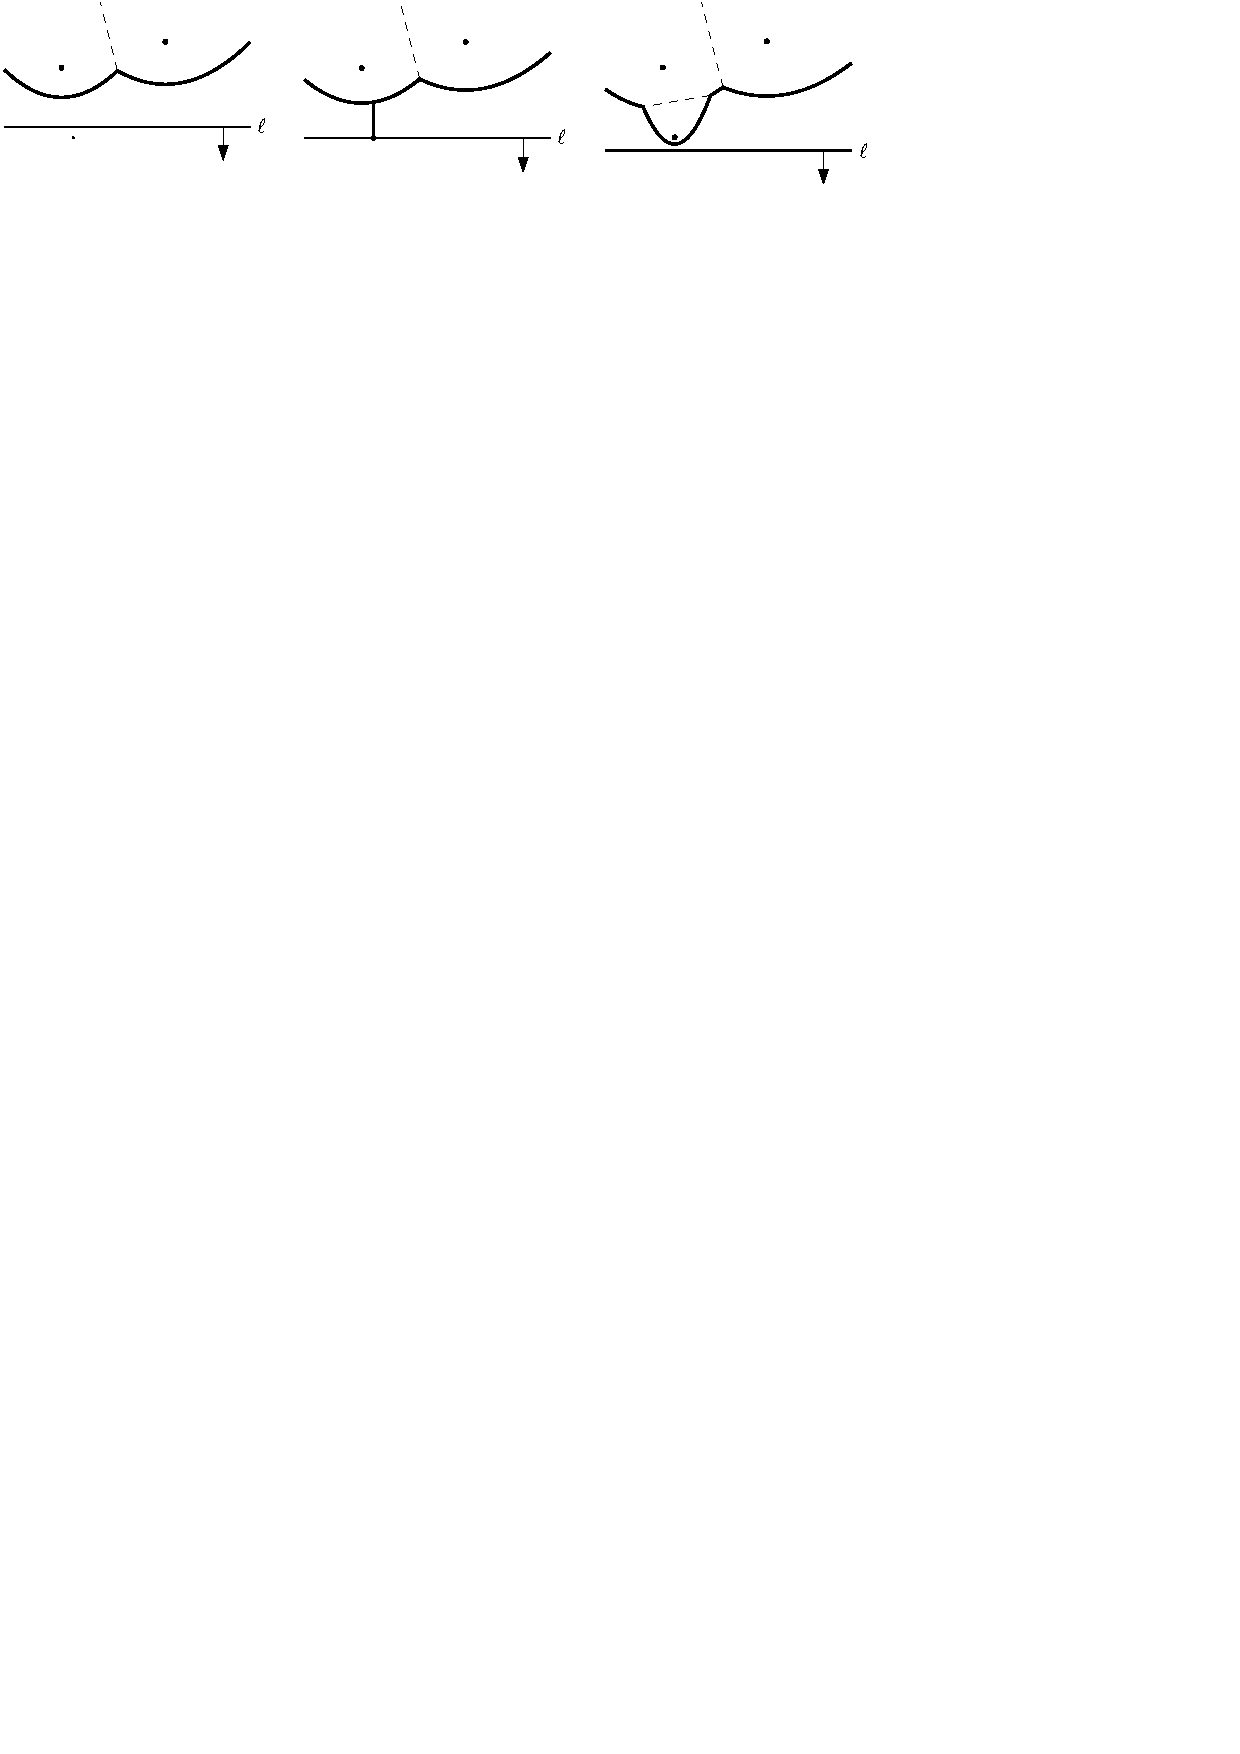
\includegraphics[width=\textwidth]{../images/siteevent}
\]
\pause
Dette kalder vi for en \textit{site begivenhed}.
\end{frame}

\begin{frame}
\pause
Vi så at der bliver fjernet en kurve fra kystlinjen når to Voronoi diagram kanter mødes.
\[
	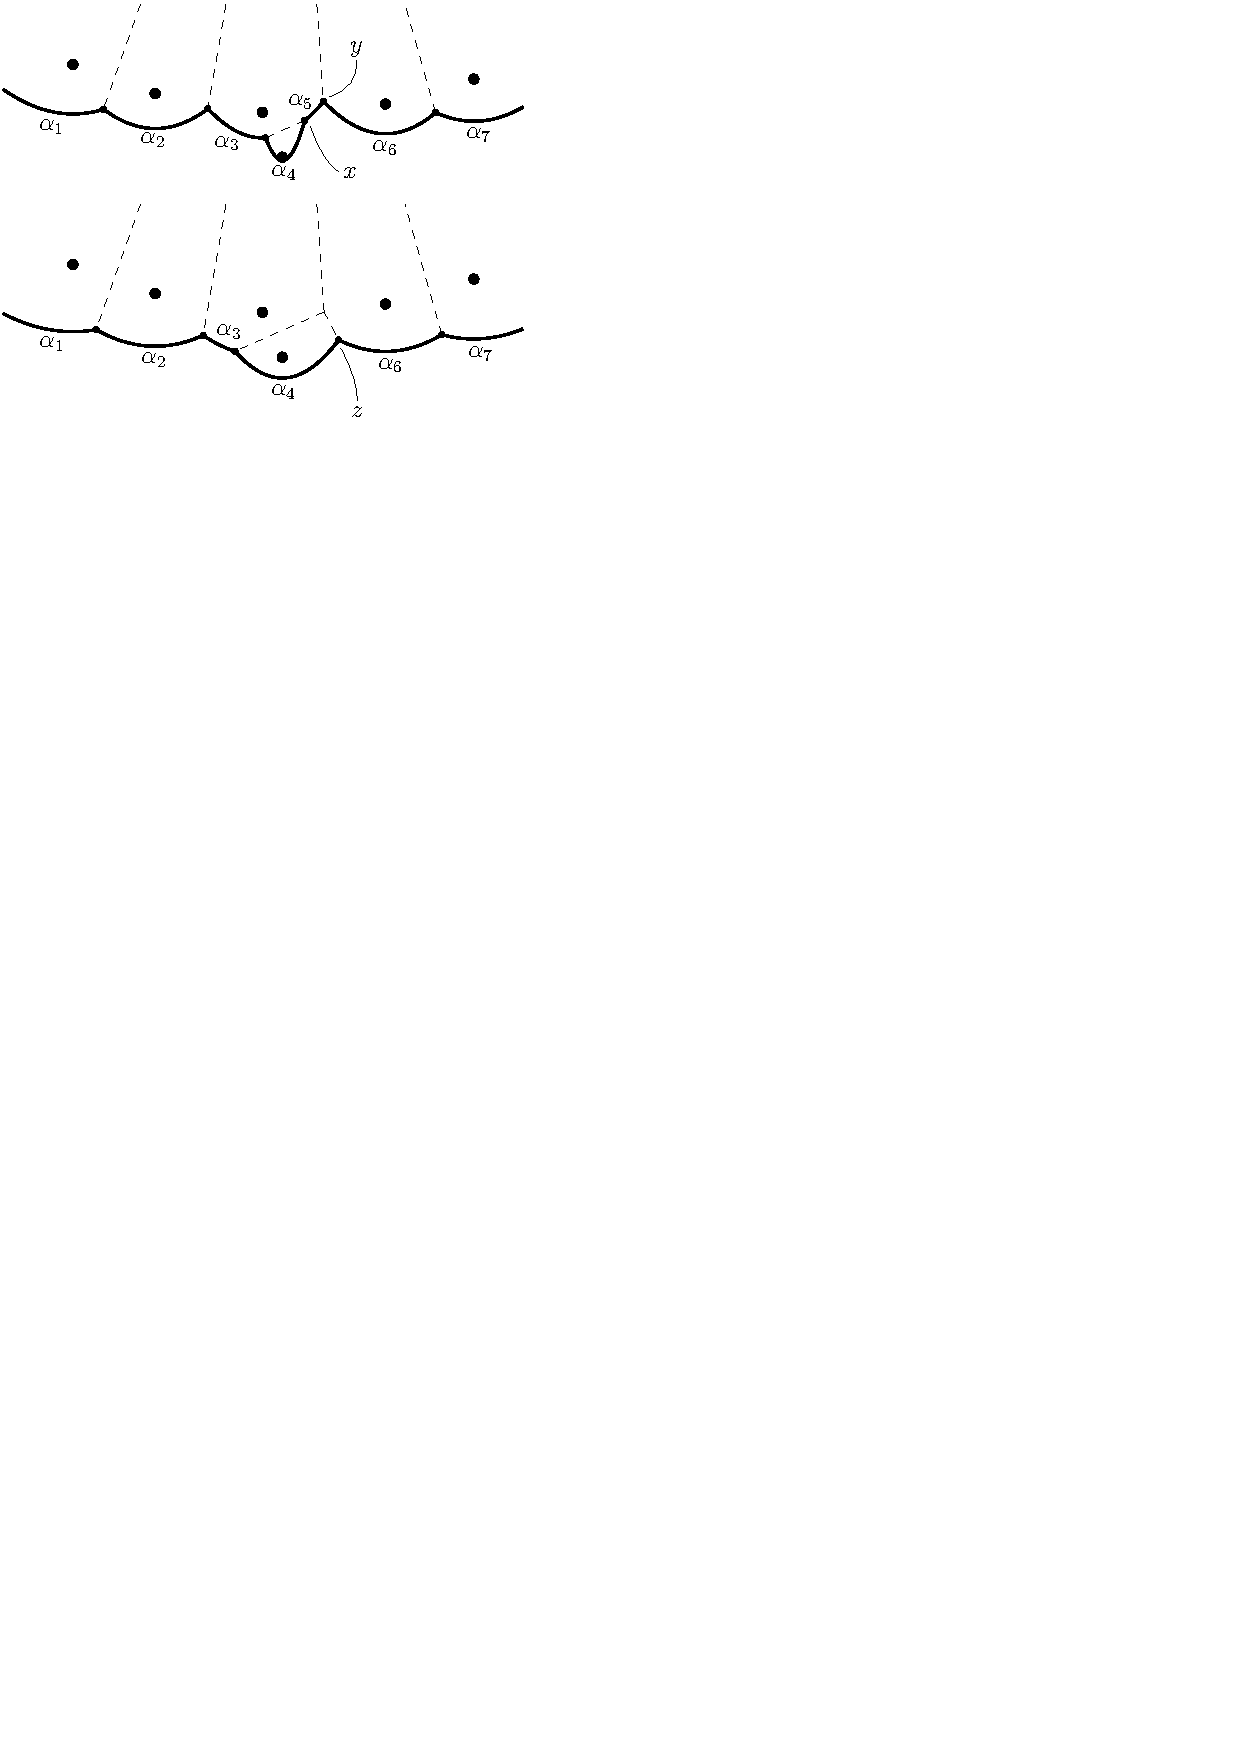
\includegraphics[scale=0.8]{../images/circle_event_beachline_merge}
\]
\pause
Dette kalder vi for en \textit{cirkel begivenhed}.\pause..indtil videre. Det er lidt mere teknisk og kommer senere.
\end{frame}

\begin{frame}
\pause
Ved en site begivenhed begynder en ny kant fra Voronoi diagrammet at vise sig.
\longpause
Ved en cirkel begivenhed bliver to kanter forbundet, og vi får en ny knude for Voronoi diagrammet, og en ny kant fortsættes.
\longpause
Når vores sweep line $\ell$ har været i gennem alle begivenhederne i ordnet rækkefølge opdager vi da hele strukturen på Voronoi diagrammet.
\end{frame}

\begin{frame}
\pause
Vi kommer til at se at for $P$ med $n$ punkter at der kun er $\mathcal{O}(n)$ site og cirkel begivenheder.
\longpause
Vi behøver altså kun at flytte $\ell$ et endeligt antal steder hen, for at opdage strukturen på Voronoi diagrammet.
\longpause
Nu til de tekniske detaljer...
\end{frame}

% % % % % % % % % % % % % % % % 
%
%
% MATEMARISK TEORI
%
%
% % % % % % % % % % % % % % % % 

\begin{frame}
\pause
\[
	\huge\text{Matematisk teori}
\]
\end{frame}

\begin{frame}
\pause
Lad $\dist(p, q)$ betegne den Euklidiske afstand mellem $p, q \in \R^2$. \pause Dvs.
\[
	\dist(p, q) = \norm{p - q}\pause, \quad \text{hvor} \quad \norm{(x, y)} = \sqrt{x^2 + y^2}.
\]
\pause
\begin{block}{Definition (Voronoi celle)}
\pause
For $p_i \in P$ definerer vi \textit{Voronoi cellen for} $p_i$ \pause til at være
\[
	\mathcal{V}(p_i) = \makeset{q \in \R^2}{\dist(q, p_i) < dist(q, p_j) \text{ for alle } i \neq j}.
\]
\end{block}
\pause
\[
	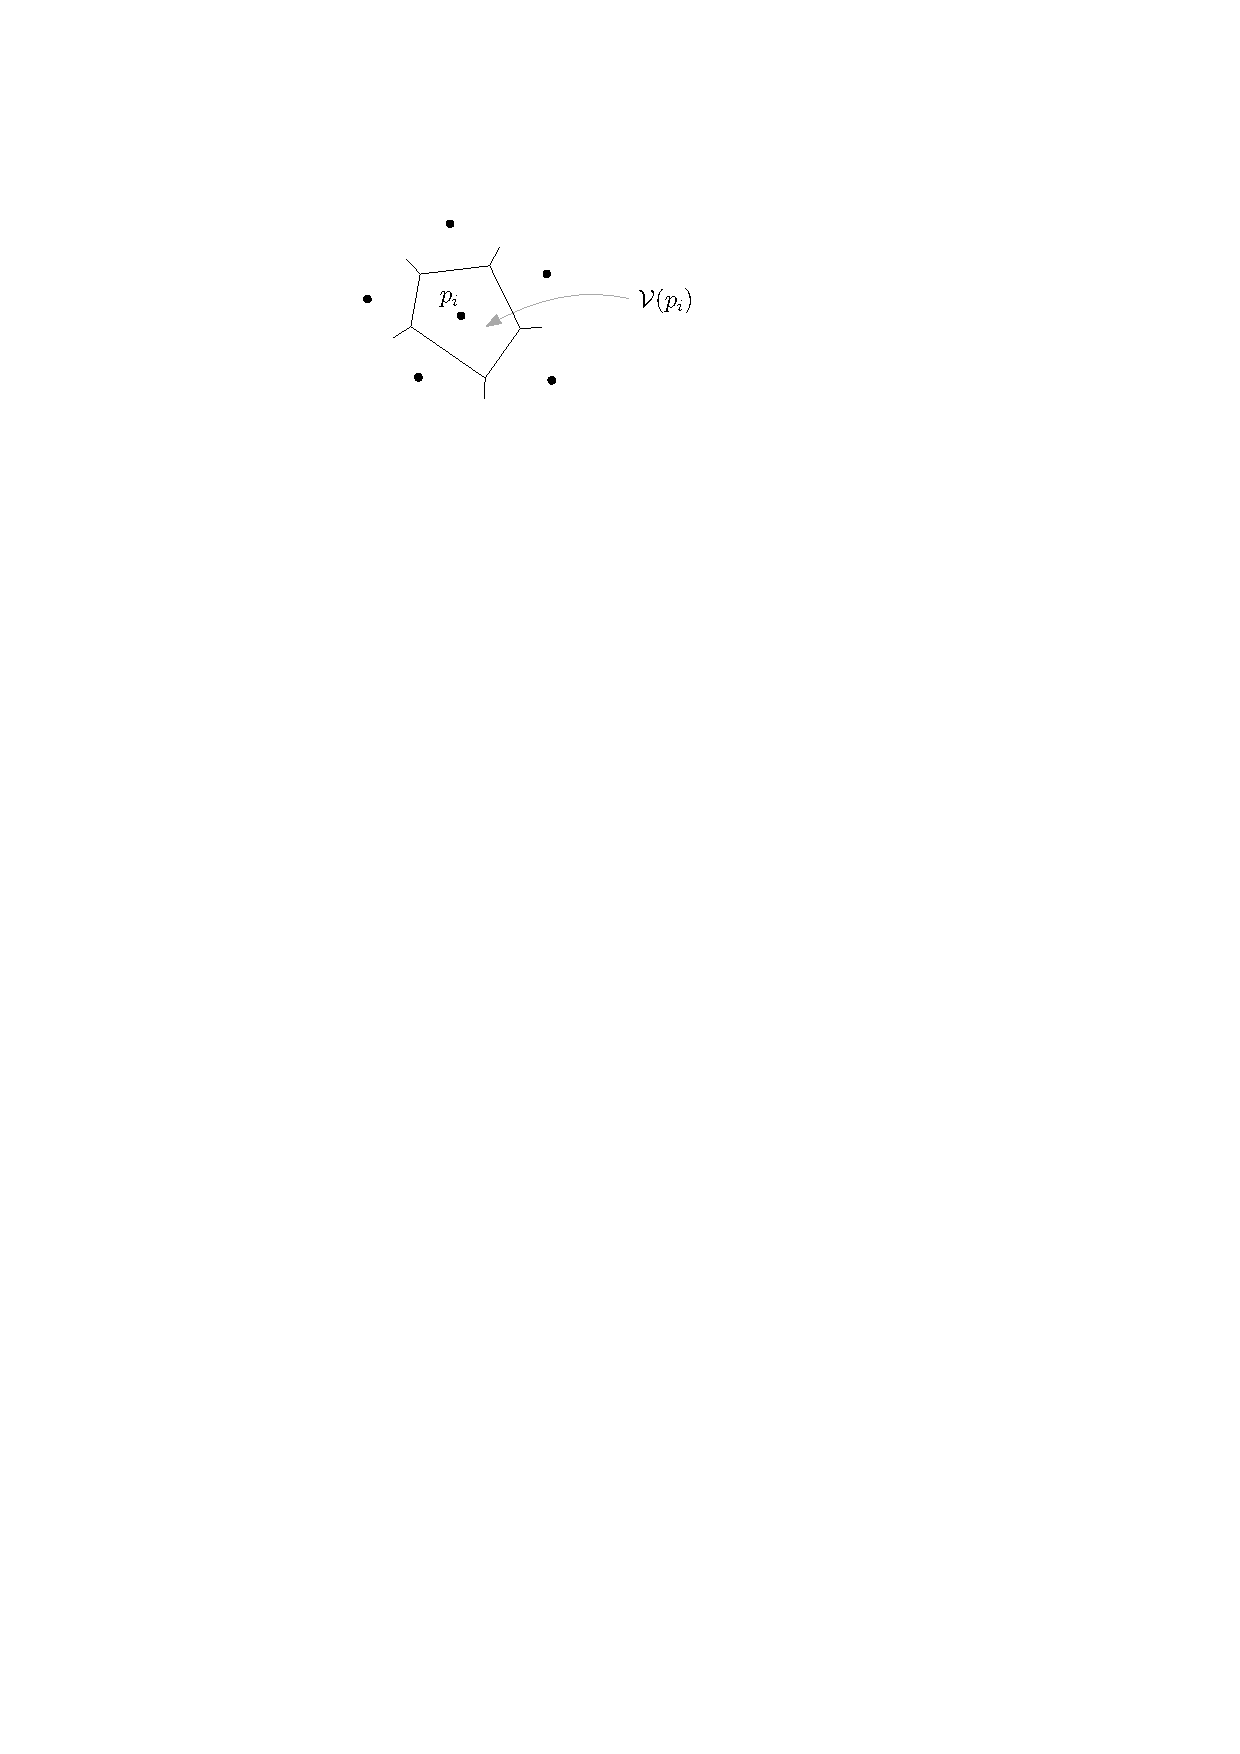
\includegraphics{images/cell_defn}
\]
\end{frame}

\begin{frame}
\pause
\begin{block}{Definition (Voronoi diagram)}
\pause
$\Vor(P) = \bigcup_{i=1}^{n} \mathcal{V}(p_i)$.
\end{block}
\pause
\begin{block}{Definition (Voronoi graph)}
\pause
$\VorG(P) = \R^2 - \Vor(P)$.
\end{block}
\pause
Strengt set, så er de knuder og kanter vi har lyst til at beregne en del af $\VorG(P)$.
\end{frame}

\begin{frame}
\pause
\begin{block}{Definition (Bisector)}
\pause
For $p, q \in \R^2$ definerer vi
\[
	\bi(p, q) = \makeset{r \in \R^2}{\dist(r, p) = \dist(r, q)}.
\]
\end{block}
\pause
En sådan bisector splitter planen i to halvplaner, $H_p$ og $H_q$.
\[
	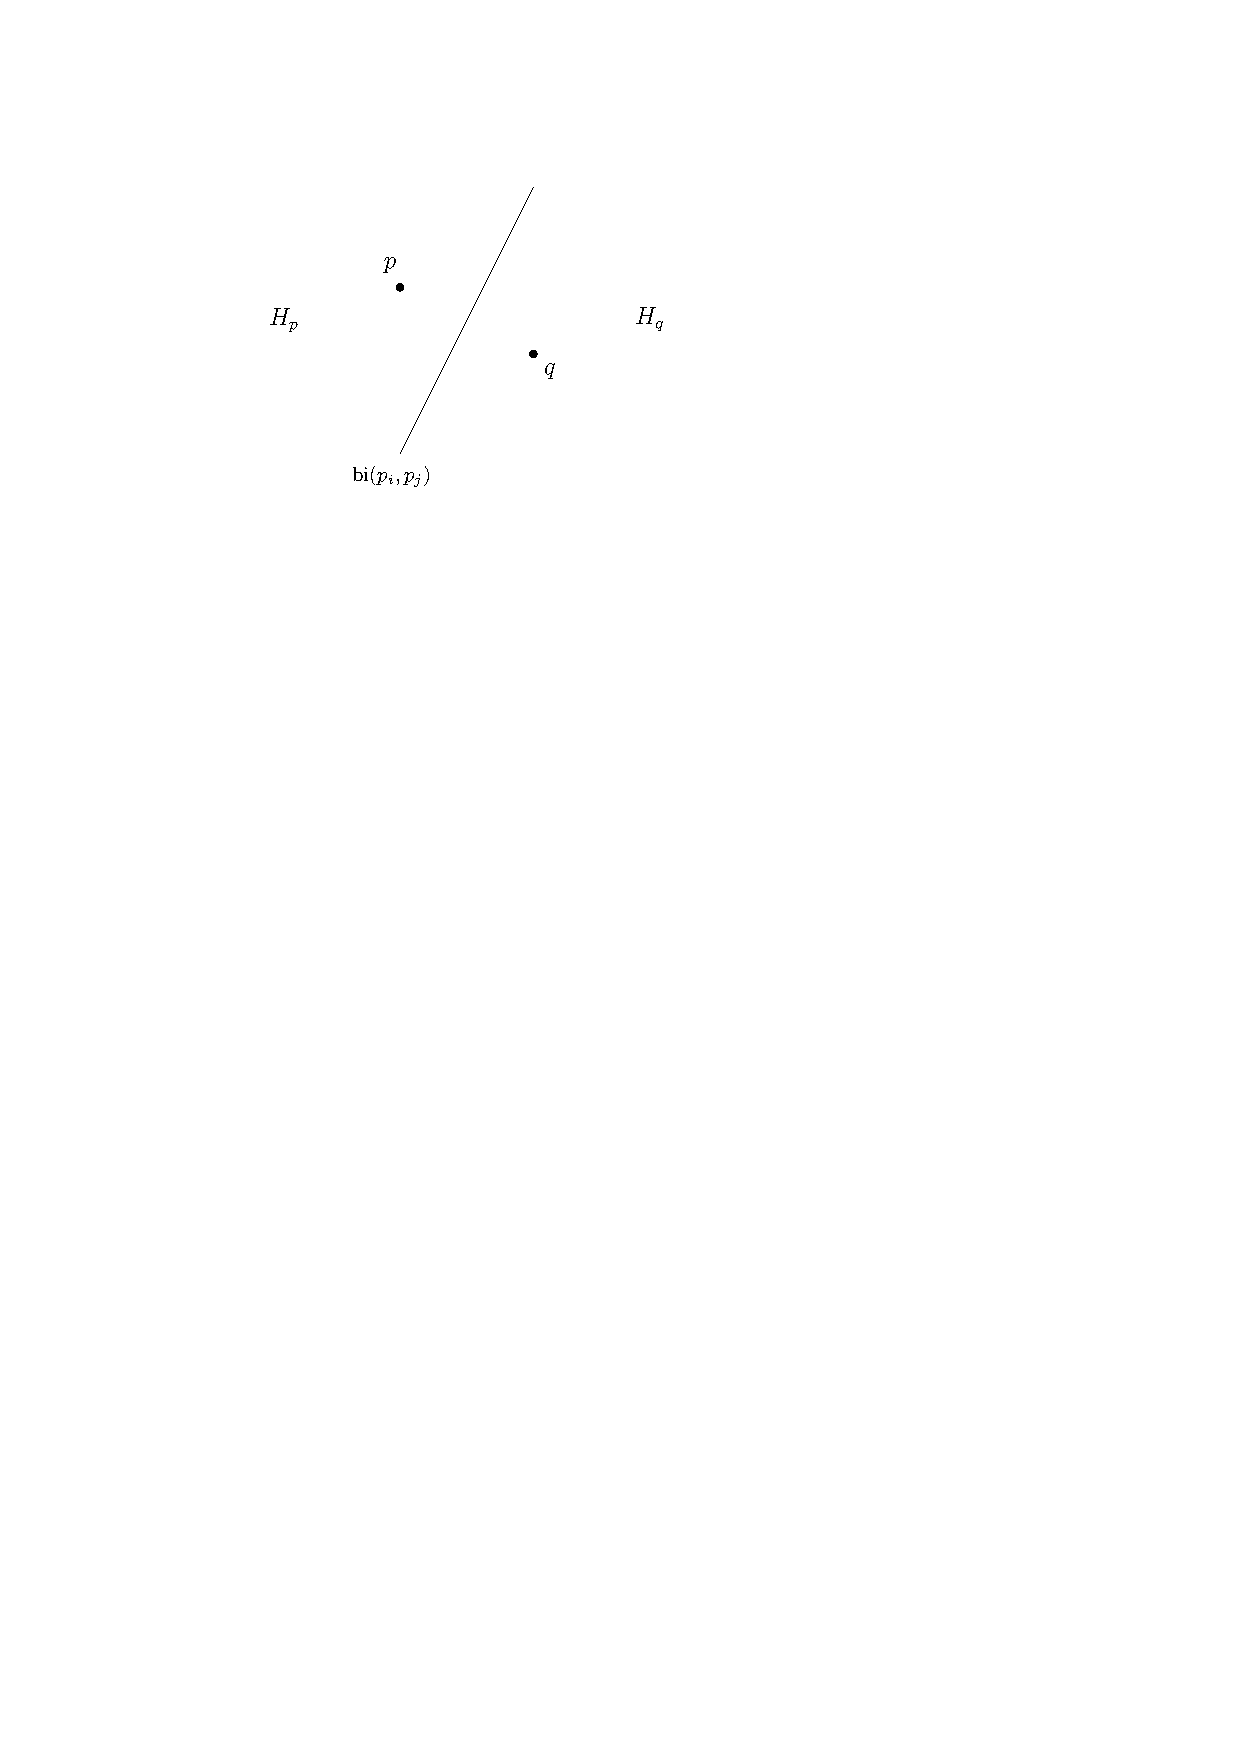
\includegraphics[scale=0.9]{../images/bisector}
\]
\end{frame}

\begin{frame}
\pause
Lad $h(p, q)$ betegne det indre af $H_p$.
\pause
\begin{block}{Proposition}
\pause
$r \in h(p, q)$ hvis og kun hvis $\dist(r, p) < \dist(r, q)$.
\end{block}
\pause
\[
	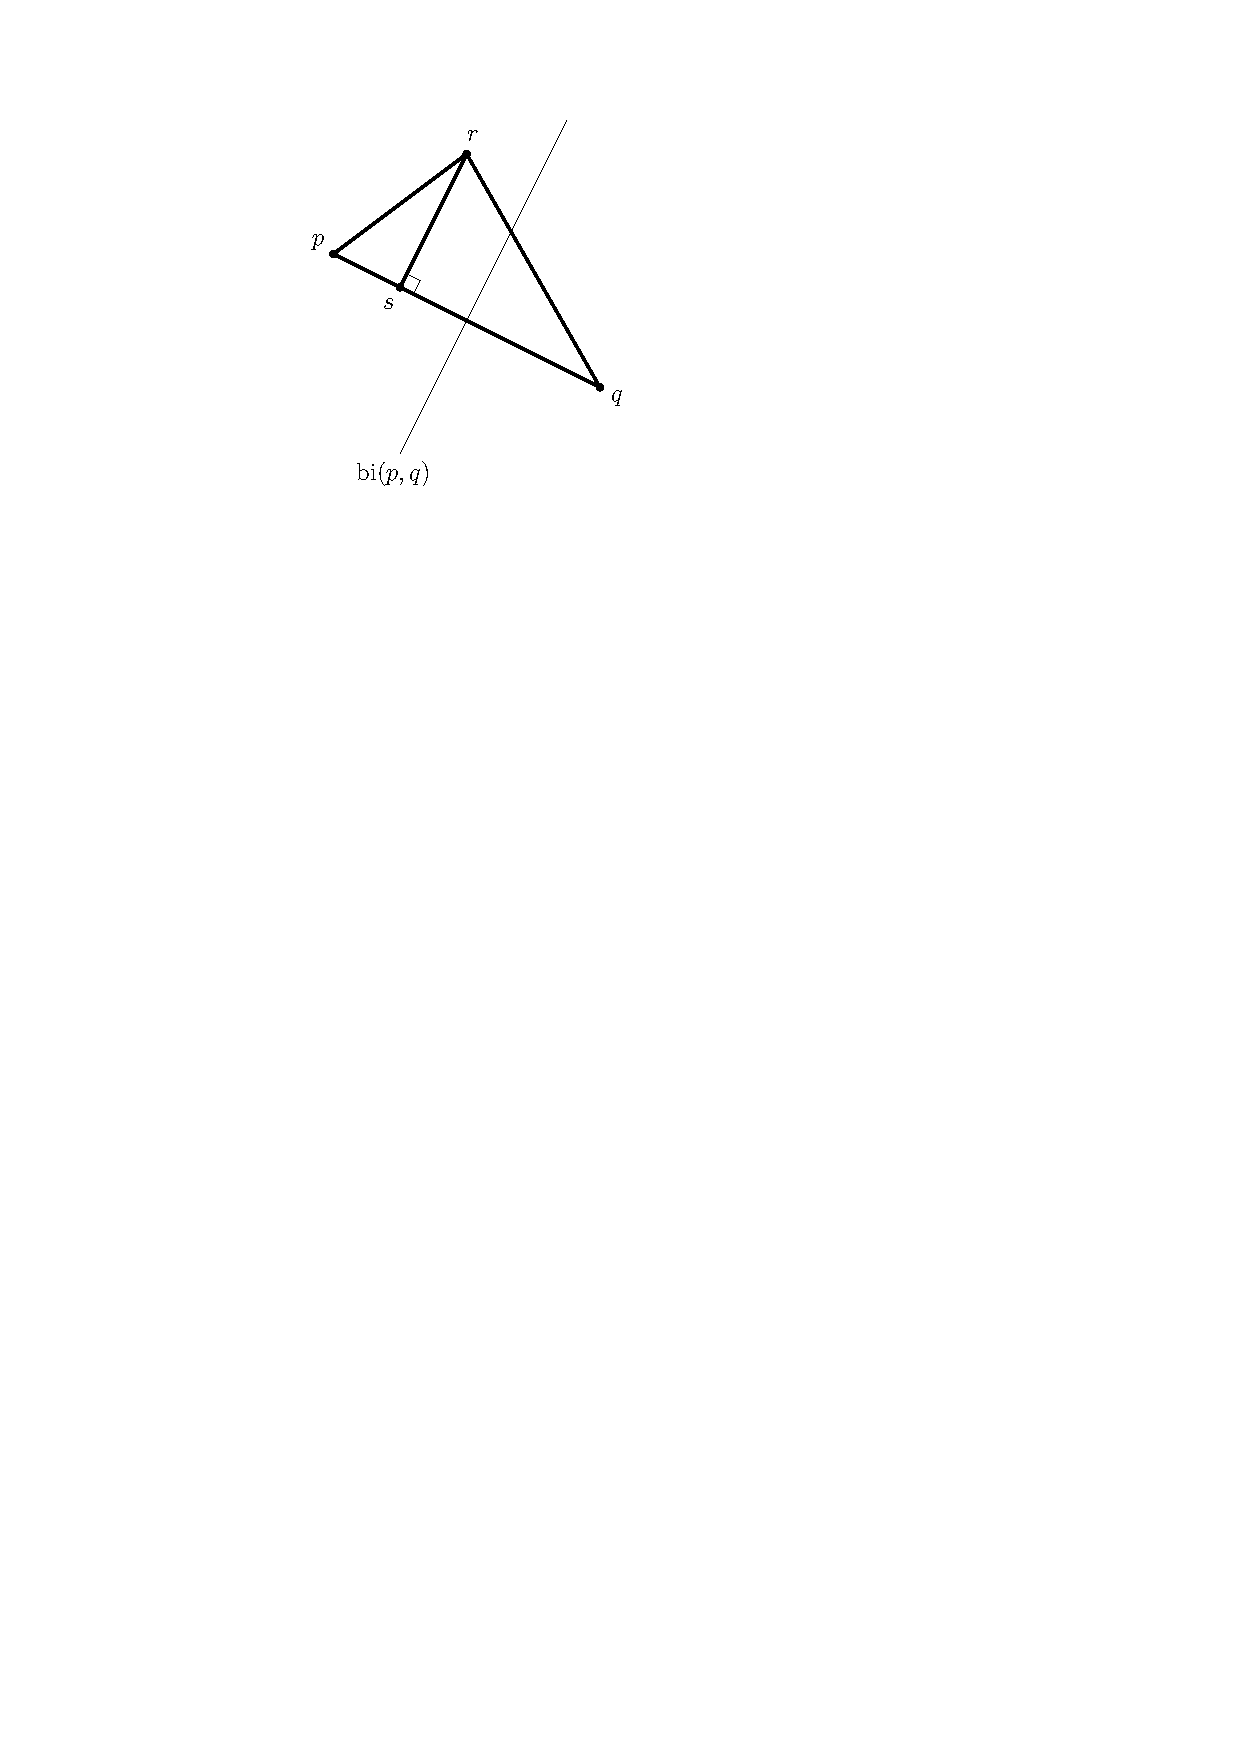
\includegraphics[scale=0.75]{../images/halfplane_containment}
\]
\pause
\vspace{-2em}
\begin{block}{Korollar 1}
\pause
$\mathcal{V}(p_i) = \bigcap_{j \ne i} h(p_i, p_j)$.
\end{block}
\end{frame}

\begin{frame}
\pause
Da $h(p_i, p_j)$ er konveks for alle $i \ne j$, har vi at $\mathcal{V}(p_i) = \bigcap_{j \ne i} h(p_i, p_j)$ også er konveks.
\longpause
Dvs. at Voronoi celler er konvekse ``polygoner'' med højst $n - 1$ knuder og højst $n - 1$ kanter.
\longpause
Nu ved vi hvordan diagrammet ser ud lokalt, men hvad med globalt?
\end{frame}

\begin{frame}
\pause
Korollar 1 giver os at $\partial \mathcal{V}(p_i)$ består af sammenhængende men muligvis tomme dele fra $\bi(p_i, p_j)$ for alle $i \ne j$.
\longpause
Dvs. at hele Voronoi diagrammet består af linjestykker, stråler og linjer, som alle ligger på forskellige bisectors $\bi(p_i, p_j)$.
\longpause
Vi viser nu:
\pause
\begin{block}{Sætning 1}
\pause
Hvis alle punkter i $P$ ligger på den samme linje, så består $\VorG(P)$ af $n - 1$ parallelle linjer.
\pause Hvis ikke, så er $\VorG(P)$ sammenhængende, og kanterne er enten linjestykker eller stråler.
\end{block}
\end{frame}

\begin{frame}
\begin{block}{Sætning 1}
Hvis alle punkter i $P$ ligger på den samme linje, så består $\VorG(P)$ af $n - 1$ parallelle linjer.
Hvis ikke, så er $\VorG(P)$ sammenhængende, og kanterne er enten linjestykker eller stråler.
\end{block}
\pause \textit{Bevis.} \pause Antag at alle punkter i $P$ ligger på den samme linje. \pause Ved at anvende en isometri på punkterne i $P$, \pause dvs. en afbildning $\varphi \colon \R^2 \to \R^2$ som opfylder at
\[
	\dist(p, q) = \dist(\varphi(p), \varphi(q))
\]
for alle $p, q \in \R^2$\pause, hvor vi bemærker at den topologiske struktur af Voronoi diagrammet dermed ikke ændres\pause, og ved dernæst at sortere punkterne\pause, kan vi uden tab af generalitet antage at
\[
	P = \curly{(x_1, 0), (x_2, 0), \ldots, (x_n, 0)},
\]
for $x_1 < x_2 < \cdots < x_n$.
\end{frame}

\begin{frame}
\begin{block}{Sætning 1}
Hvis alle punkter i $P$ ligger på den samme linje, så består $\VorG(P)$ af $n - 1$ parallelle linjer.
Hvis ikke, så er $\VorG(P)$ sammenhængende, og kanterne er enten linjestykker eller stråler.
\end{block}
\textit{Bevis fortsat.} \pause Lad $(x, y) \in \R^2$ så $x_i < x < x_{i+1}$ for et $i < n$. \pause Bemærk så at hvis $(x,y) \in \VorG(P)$ \pause så gælder at
\begin{align*}
	&\norm{(x, y) - (x_i, 0)} = \norm{(x, y) - (x_{i+1}, 0)} \\ \Pause
	\iff &\sqrt{(x - x_i)^2 + y^2} = \sqrt{(x - x_{i+1})^2 + y^2} \\ \Pause
	\iff &\abs{x - x_i} = \abs{x - x_{i+1}}.
\end{align*}
\Pause
Dvs. at hvis $(x, 0) \in \VorG(P)$ så er $(x, y) \in \VorG(P)$ for alle $y \in \R$.
\longpause
Det følger at $\VorG(P) = \bigcup_{i=1}^{n - 1} \bi((x_i, 0), (x_{i+1}, 0))$, og disse er alle parallelle linjer.
\end{frame}

\begin{frame}
\begin{block}{Sætning 1}
Hvis alle punkter i $P$ ligger på den samme linje, så består $\VorG(P)$ af $n - 1$ parallelle linjer.
Hvis ikke, så er $\VorG(P)$ sammenhængende, og kanterne er enten linjestykker eller stråler.
\end{block}
\textit{Bevis fortsat.} \pause Antag nu at punkterne i $P$ ikke ligger på den samme linje. \pause Vi viser først at alle kanterne i $\VorG(P)$ enten er linjestykker eller stråler. \pause
\vspace{0.5em}
\begin{columns}
\begin{column}{0.5\textwidth}
	\begin{center}
		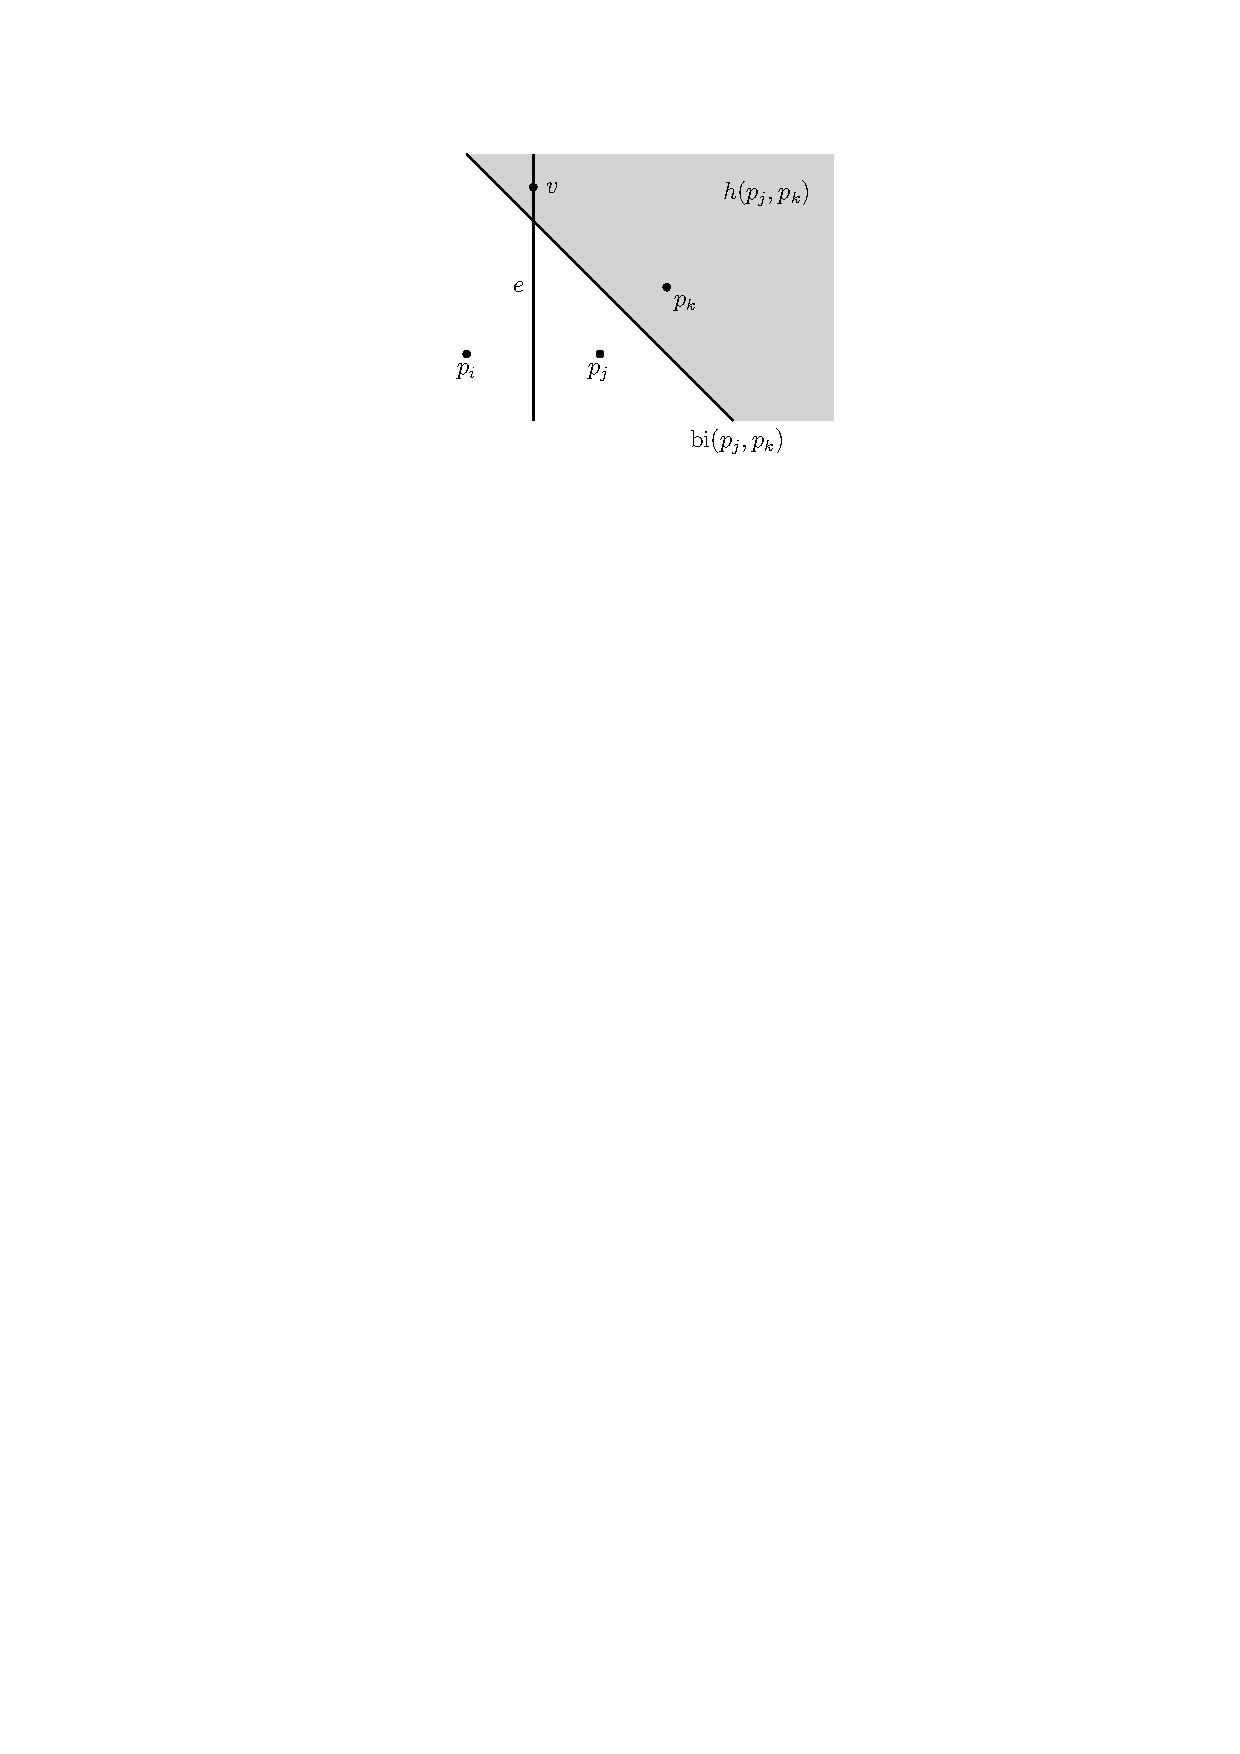
\includegraphics[scale=0.8]{../images/diagram_is_connected}
	\end{center}
\end{column}
\begin{column}{0.5\textwidth}
    Antag for modstrid at dette ikke er tilfældet\pause, hvormed der findes en kant $e \subset \partial \mathcal{V}(p_i) \cap \partial \mathcal{V}(p_j)$ som er en hel linje. \pause Lad $p_k$ være et punkt som ikke ligger på $\overline{p_i p_j}$. \pause Så er $\bi(p_j, p_k)$ og $e$ ikke parallelle\pause, hvormed de har et skæringspunkt. \pause Dette giver at der findes et punkt $v \in e \cap {}^{\circ}h(p_k, p_j)$.
\end{column}
\end{columns}
\end{frame}

\begin{frame}
\begin{block}{Sætning 1}
Hvis alle punkter i $P$ ligger på den samme linje, så består $\VorG(P)$ af $n - 1$ parallelle linjer.
Hvis ikke, så er $\VorG(P)$ sammenhængende, og kanterne er enten linjestykker eller stråler.
\end{block}
\textit{Bevis fortsat.} \pause Så $v \in \partial \mathcal{V}(p_i) \cap \partial \mathcal{V}(p_j) \cap {}^{\circ}h(p_k, p_j)$. \pause Da $v \in h(p_k, p_j)$ har vi at
\[
	\dist(v, p_k) < \dist(v, p_j).
\]
\pause Men da $v \in \partial \mathcal{V}(p_j)$ gælder
\[
	\dist(v, p_k) \geq \dist(v, p_j), \pause
\]
og vi har en modstrid. \pause (Bemærk fejl i speciale på s. 8!)
\end{frame}

\begin{frame}
\begin{block}{Sætning 1}
Hvis alle punkter i $P$ ligger på den samme linje, så består $\VorG(P)$ af $n - 1$ parallelle linjer.
Hvis ikke, så er $\VorG(P)$ sammenhængende, og kanterne er enten linjestykker eller stråler.
\end{block}
\textit{Bevis fortsat.} \pause Vi viser nu at $\VorG(P)$ er sammenhængende. \pause Antag for modstrid at $\VorG(P)$ ikke er sammenhængende. \pause Så findes $\partial \mathcal{V}(p_i)$ som ikke er stisammenhængende. \pause Det kan kun ske hvis $\partial \mathcal{V}(p_i)$ består af to parallelle linjer\pause, hvilket er i modstrid med at $\VorG(P)$ ikke indeholder nogen linjer. \pause Altså er $\VorG(P)$ sammenhængende. \textbf{QED.}
\end{frame}

\begin{frame}
\pause
Vi viser nu at antallet af knuder og kanter i $\VorG(P)$ er $\mathcal{O}(n)$.
\pause
\begin{block}{Sætning 2}
\pause
For $n \geq 3$ er antallet af knuder i $\VorG(P)$ højst $2n - 5$ \pause og antallet af kanter er højst $3n - 6$.
\end{block}
\pause \textit{Bevis.} \pause Hvis punkterne i $P$ alle ligger på den samme linje, så giver Sætning 1 at $\VorG(P)$ opfylder de angivne øvre grænser.
\longpause
Antag nu at punkterne i $P$ ikke alle ligger på den samme linje. \pause Vi vil benytte Eulers formel, som for en plan graf med \pause $V$ knuder, \pause $E$ kanter \pause og $F$ sideflader \pause siger at
\[
	V - E + F = 2.
\]
\pause Vi har dog det problem at $\VorG(P)$ ikke er en plan graf i ovenstående forstand, da den har nogle uendelige kanter. \pause Vi laver nu en transformation af $\VorG(P)$ som gør at vi kan benytte formlen.
\end{frame}

\begin{frame}
\begin{block}{Sætning 2}
For $n \geq 3$ er antallet af knuder i $\VorG(P)$ højst $2n - 5$ og antallet af kanter er højst $3n - 6$.
\end{block}
\textit{Bevis fortsat.} \pause Lad $v_1, v_2, \ldots, v_k$ være knuderne i $\VorG(P)$. \pause Lad
\[
	p = \frac{1}{k} (v_1 + v_2 + \cdots + v_k) \in \R^2
\]
\pause og
\[
	r = 1 + \max\curly{\dist(p, v_1), \ldots, \dist(p, v_k)}. \pause
\]
Vi har så at $v_1, \ldots, v_k \in B_r(p)$ \pause og enhver kant i $\VorG(P)$ som er en stråle skærer $\partial B_r(p)$ i et entydigt punkt\pause, kald disse punkter $s_1, s_2, \ldots, s_t$. \pause Definér så $v_{\infty}$ som et vilkårligt element i $\R^2 \setminus \overline{B_r(p)}$. \pause Vi kan så forbinde enhver uendelig kant til $v_{\infty}$\pause, ved at forbinde $s_i$ til $v_{\infty}$ med en sti\pause, og vi gør det i rækkefølge, startende med det $s_i$ som ligger tættest på $v_{\infty}$.
\end{frame}

\begin{frame}
Et eksempel på denne konstruktion er givet her:
\pause
\[
	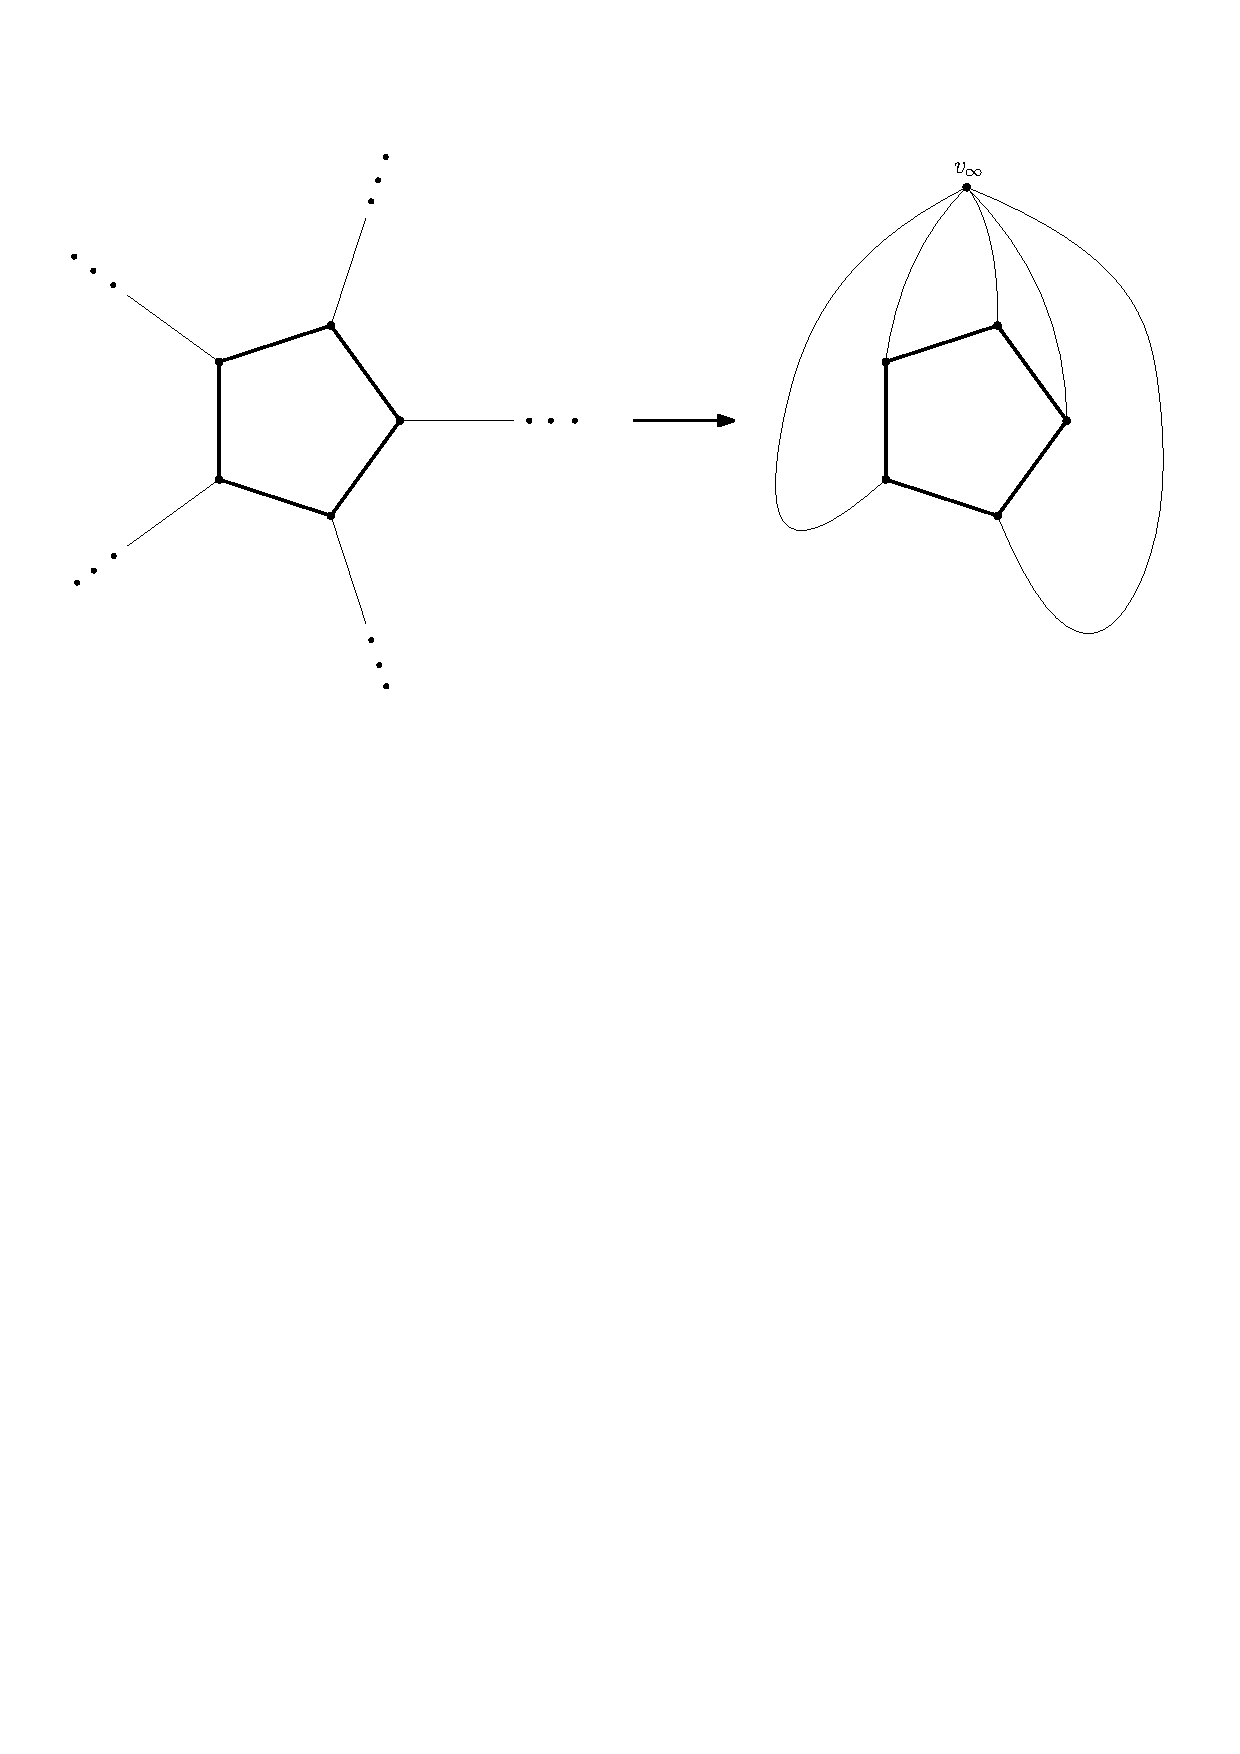
\includegraphics[width=\textwidth]{../images/projective_embedding}
\]
\end{frame}

\begin{frame}
\begin{block}{Sætning 2}
For $n \geq 3$ er antallet af knuder i $\VorG(P)$ højst $2n - 5$ og antallet af kanter er højst $3n - 6$.
\end{block}
\textit{Bevis fortsat.} \pause Lad $G$ være grafen der fremkommer ved at transformere $\VorG(P)$. \pause Vi kan nu anvende Eulers formel på $G$. \pause Lad $n_v$ betegne antallet af knuder i $\VorG(P)$, og lad $n_e$ betegne antallet af kanter. \pause Antallet af sideflader er $n$, da vi har én Voronoi celle for hvert site. \pause Vi har kun tilføjet en enkelt knude, så ved indsættelse i Eulers formel får vi
\begin{equation} \label{eq:eulerapplied}
	(n_v + 1) - n_e + n = 2.
\end{equation}
\pause Bemærk så, at enhver knude $v$ i $G$ har $\deg(v) \geq 3$\pause, for ellers ville der være en $\mathcal{V}(p_i)$ som ikke er konveks. \pause Dvs.
\[
	\sum_{v \in V(G)} \deg(v) \pause \geq 3 \abs{V(G)} \pause = 3 (n_v + 1).
\]
\pause Vi finder nu et udtryk for venstresiden.
\end{frame}

\begin{frame}
\begin{block}{Sætning 2}
For $n \geq 3$ er antallet af knuder i $\VorG(P)$ højst $2n - 5$ og antallet af kanter er højst $3n - 6$.
\end{block}
\textit{Bevis fortsat.} \pause Bemærk at $\deg(v)$ tæller antallet af kanter som rører $v$\pause, og i $G$ så rører hver kant ved præcis $2$ knuder\pause, så $\sum_{v \in V(G)} \deg(v) = 2 n_e$. \pause Dvs.
\begin{equation} \label{eq:eulerineq}
	2 n_e \geq 3 (n_v + 1).
\end{equation}
\pause Vi får så:
\begin{align*}
	&2 (n_v + 1) - 2 n_e + 2n = 4 \quad \text{(Gang (\ref{eq:eulerapplied}) med 2)} \\ \Pause
	\iff &2 n_e = (2 n_v + 1) + 2n - 4 \quad \text{(Isolér $2 n_e$)} \\ \Pause
	\implies &3 (n_v + 1) \leq 2 (n_v + 1) + 2n - 4 \quad \text{(Anvend (\ref{eq:eulerineq}))} \\ \Pause
	\implies &n_v \leq 2n - 5.
\end{align*}
\pause Altså er antallet af knuder højst $2n - 5$.
\end{frame}

\begin{frame}
\begin{block}{Sætning 2}
For $n \geq 3$ er antallet af knuder i $\VorG(P)$ højst $2n - 5$ og antallet af kanter er højst $3n - 6$.
\end{block}
\textit{Bevis fortsat.} \pause Mht. kanterne har vi:
\begin{align*}
	&3 (n_v + 1) - 3 n_e + 3n = 6 \quad \text{(Gang (\ref{eq:eulerapplied}) med 3)} \\ \Pause
	\iff &3(n_v + 1) = 3n_e - 3n + 6 \quad \text{(Isoler $3 (n_v + 1)$)} \\ \Pause
	\implies &2 n_e \geq 3 n_e - 3n + 6 \quad \text{(Anvend (\ref{eq:eulerineq}))} \\ \Pause
	\implies &n_e \leq 3n - 6.
\end{align*}
\pause Altså er antallet af kanter højst $3n - 6$. \pause \textbf{QED.}
\end{frame}

\end{comment}

\begin{frame}
\pause
Vi har altså set at selvom vi har $\mathcal{O}(n^2)$ bisectors, så har vi kun $\mathcal{O}(n)$ kanter. \pause Vi vil nu karakterisere hvornår en del af en bisector faktisk udgør en knude eller kant i $\VorG(P)$.
\end{frame}

\begin{frame}
\begin{block}{Definition (Største tomme cirkel)}
\pause
For $q \in \R^2$ \pause definerer vi $C_P(q)$ til at være \textit{den største tommel cirkel for $q$ mht. $P$}\pause, givet ved
\[
	C_P(q) = B_r(q)\pause, \quad \text{hvor} \quad r = \sup\makeset{\lambda \in \R^{+}}{B_{\lambda}(q) \cap P = \emptyset}.
\]
\end{block}
\pause
\[
	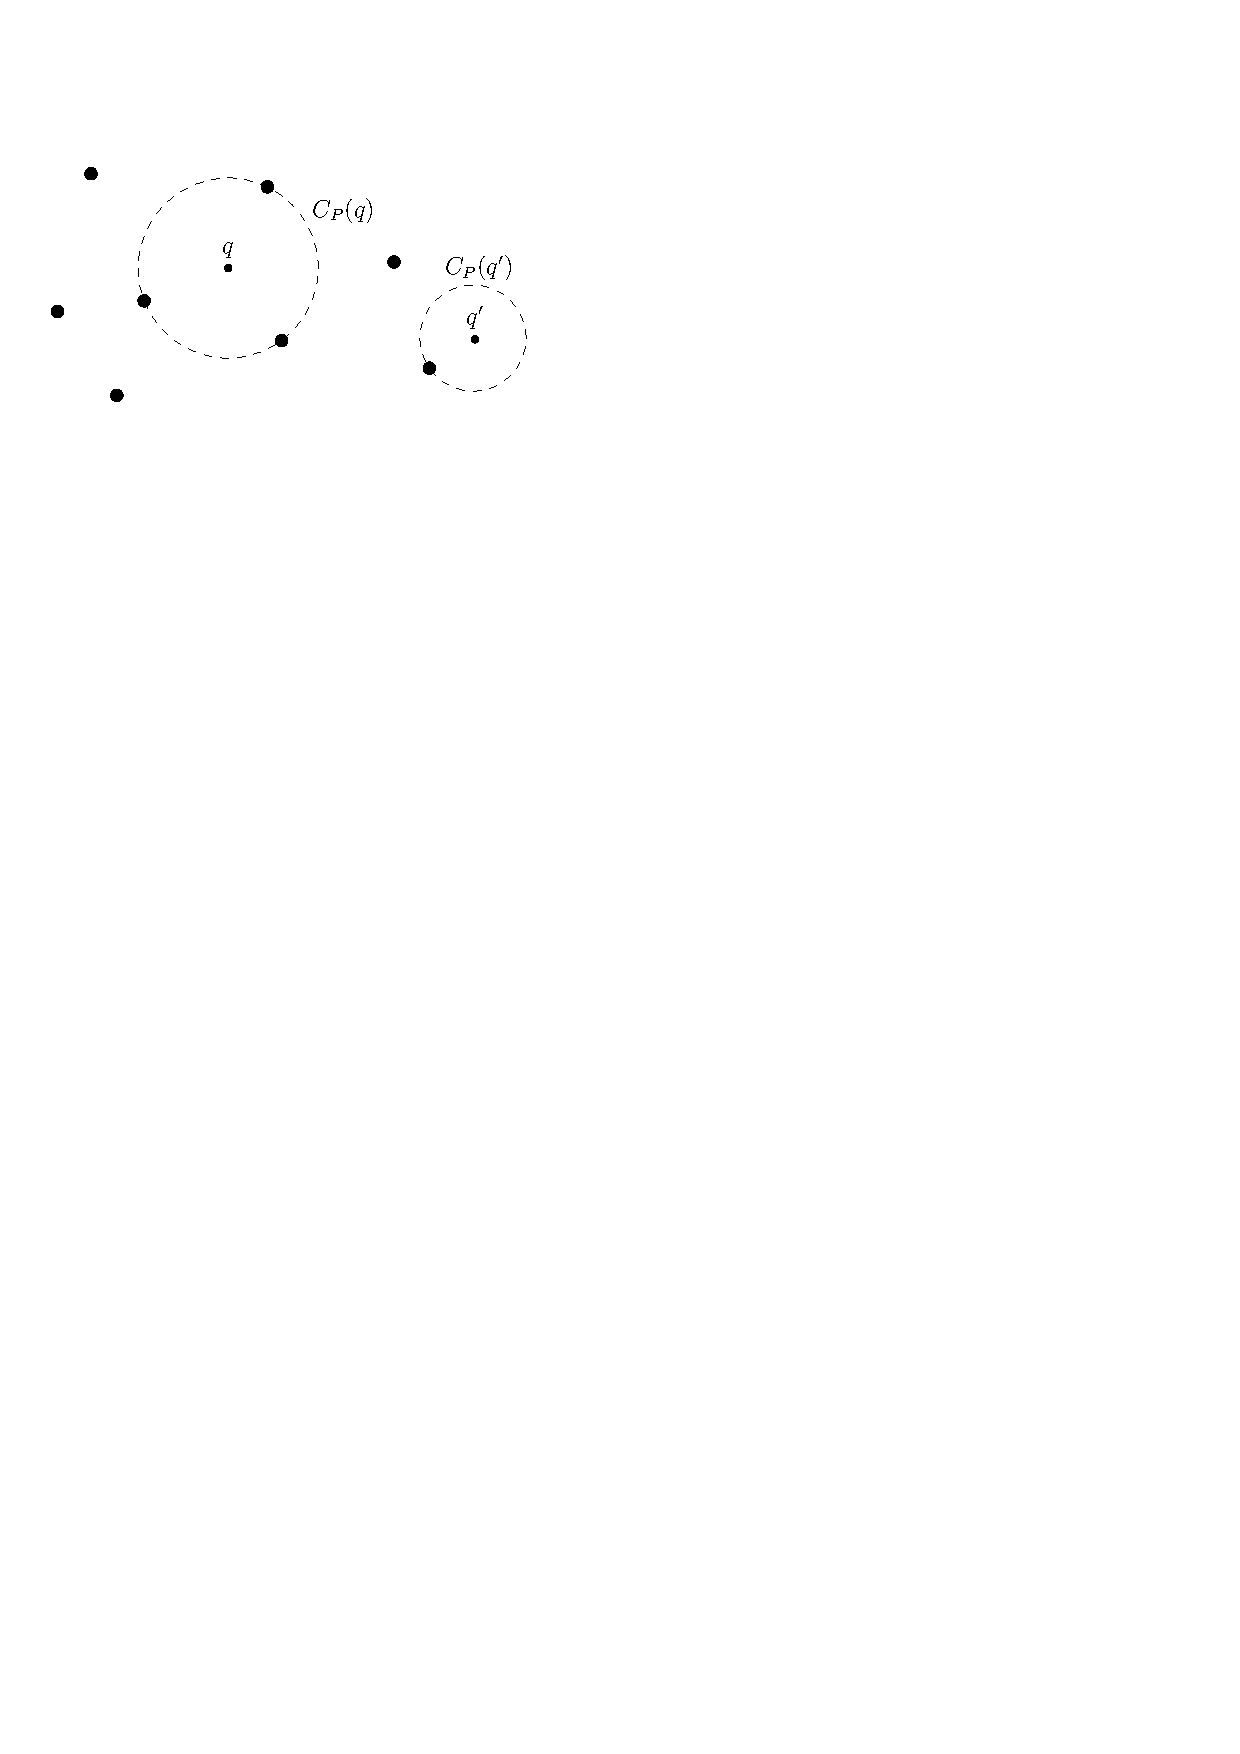
\includegraphics[scale=0.85]{../images/largest_empty_circle}
\]
\end{frame}

\begin{frame}
\pause
\begin{block}{Sætning 3}
\pause
Vi har følgende:
\begin{enumerate}
	\pause \item $q \in \R^2$ er en knude i $\VorG(P)$ \pause hvis og kun hvis
	\[
		\abs{\partial C_P(q) \cap P} \geq 3.
	\]
	\pause \item $\bi(p_i, p_j)$ definerer en kant i $\VorG(P)$ \pause hvis og kun hvis
	\[
		\exists q \in \bi(p_i, p_j) \colon \partial C_P(q) \cap P = \curly{p_i, p_j}.
	\]
\end{enumerate}
\end{block}
\longpause
Beviset består af nogle simple observationer og modstrider, så vi præsenterer det ikke her. \pause Denne figur bør give den intuition som er nødvendig:
\end{frame}

\begin{frame}
\[
	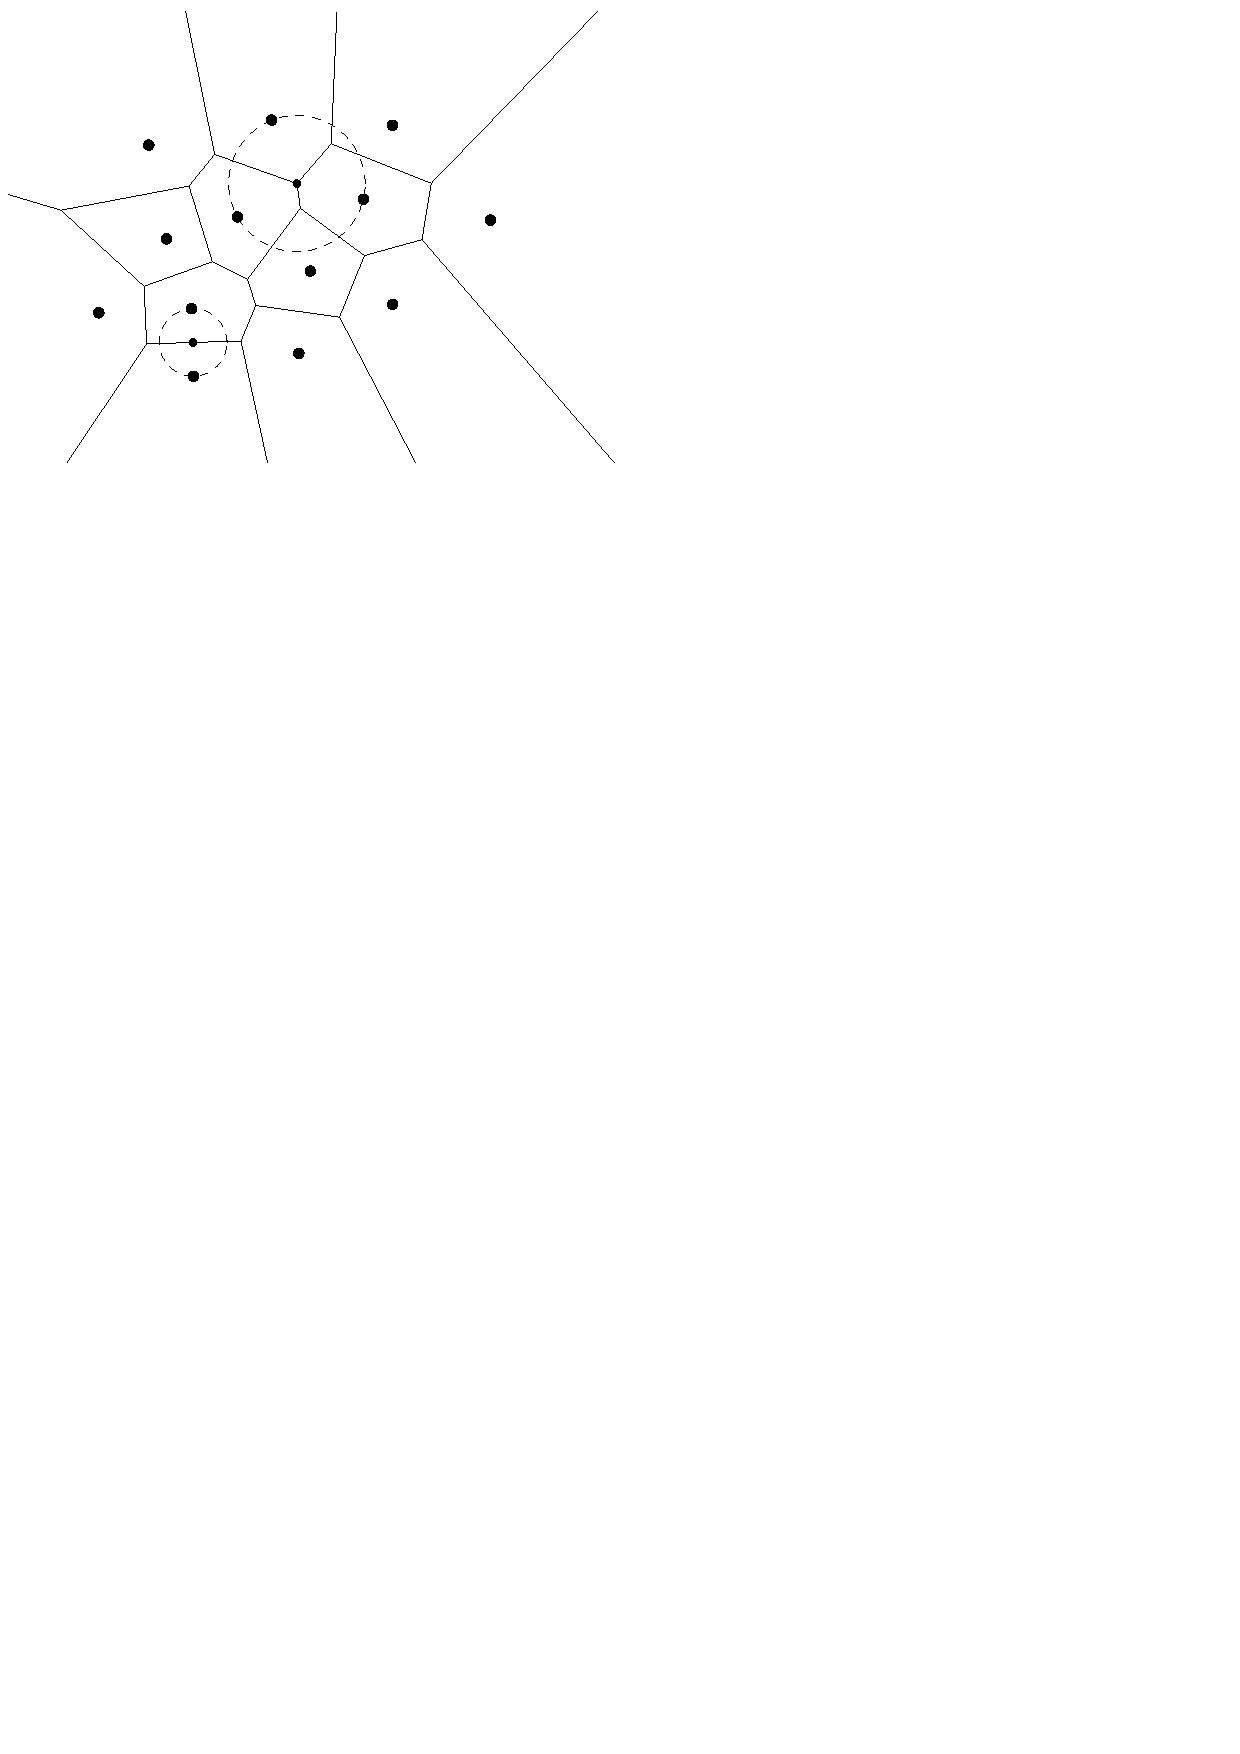
\includegraphics[scale=1.0]{../images/vert_edge_char}
\]
\end{frame}

\begin{frame}
\pause
Hej
\end{frame}

\end{document}